\subsection{Two Step Fitter Validation}
\label{sec:OptimizationThenFitValidation}

As a reference, we document the validation procedure for the fit
performed in two steps: 1) determining the optimal fractions of Matching and
Scaling MC in the W$jj$ sample, 2) fitting for the yields. Specifically,
we verify that the signal extraction procedure is unbiased and that 
statistical uncertainties reported have good coverage by performing 
a number of pseudo experiments. The specific steps are:
\begin{enumerate}
\item Perform the default fit and obtain the expected yields 
(Table~\ref{table:FitValidation_2Step_input}).
\item Generate toy Monte Carlo for each process from the corresponding MC distributions.
\item Construct 1000 sample datasets with the event counts smeared according 
to a Poisson distribution.
\item Repeat the optimization procedure (to obtain the fraction of 
the ScaleUp and MatchingUp events) for each sample dataset.
\item Take the resultant optimal values (for ScaleUp and MatchingUp 
fractions) and fit for the yields.
\item Examine the resultant yields.
\end{enumerate}
Similarly to the default fit, we perform the validation for the 
2- and 3-jet bins independently. The results are
shown in Figs~\ref{fig:Validation_2j},~\ref{fig:Validation_3j},
and gaussian fits to the distributions are summarized in 
Table~\ref{table:FitValidation_2Step_results}. Note that there
is substantial variation in the gaussian widths due to differing
constraints imposed when fitting (Table~\ref{tab:mjj_shapes_and_normalization}).
There is a $-151$ event bias for the QCD
in the 2-jet bin, while for the rest of the processes the yields returned by the fitter 
are consistent with the expectation within $2\%$.


\subsubsection{Optimization Procedure Validation}
In addition to extracting the yields, we obtain the W$jj$ pull distributions 
(Fig.~\ref{fig:Validation_PullsWjj}). Since each
dataset is used to obtain the optimal values for the fraction of ScaleUp and 
MatchingUp events, the W$jj$ template already contains information from it. Thus, there
is a smaller spread in the extracted yields, as the pull $\sigma$s ($0.404\pm 0.009$ 
for the 2-jet bin and $0.685\pm 0.017$ for the 3-jet bin) indicate.

The fractions for the matchingUp and scaleUp events, obtained from the optimization
procedure, are shown in Fig.~\ref{fig:Validation_fSUfMU}.
For reference, we show the comparison between the Up and Down shapes in 
Figure~\ref{fig:Validation_ShapeComparisonUpVsDown}. Due to insufficient discriminating
ability, for the 2-jet bin, $\sim 15\%$ of the experiments produce
scaleDown events despite starting with the scaleUp sample. The effect exists, but
occurs less than $2\%$ of the time, in the case of the matching samples. In the 3-jet bin, the shapes are
sufficiently distinct to avoid such bifurcation. In the end, results of the validation
are consistent with the expectations, as well as with observations from other studies.


%%%%%%%%%%%%%%%%%%%%%%%%%%%%
%%%%%%%
\begin{table}[tb]
\caption{Yields used as inputs to generate pseudo experiments for fit validation studies.}
\begin{center}
\begin{tabular}{|c|c|c|}
\hline
   Process           & 2-Jet bin & 3-Jet bin \cr \hline
\vspace{-0.5cm} & & \cr
{Diboson}            &      1004 &  242  \cr \hline
{W$jj_{Default}$}    &     14903 & 8465  \cr \hline
{W$jj_{ScaleUp}$}    &      7488 &  737  \cr \hline
{W$jj_{MatchingUp}$} &     13781 &  629  \cr \hline
{QCD}                &      1368 &  159  \cr \hline
{$t\bar{t}$}         &      3120 &  308  \cr \hline
{Single top}         &      1182 &  652  \cr \hline
{Z+jets}             &       797 &  260  \cr \hline
\end{tabular}
\end{center}
\label{table:FitValidation_2Step_input}
\end{table}
%%%%%%%
%%%%%%%
\begin{table}[tb]
\caption{Fit Validation Summary}
\begin{center}
\begin{tabular}{|c|c|c|c|c|}
\hline
   Yields (Fitted-Expected)
 & 2-Jet Mean
 & 2-Jet $\sigma$
 & 3-Jet Mean
 & 3-Jet $\sigma$ \cr
\hline
\vspace{-0.5cm} & & \cr
{Diboson} & $-43.995\pm 1.680$ & $51.607\pm 1.330$ & $2.003\pm 0.126$ & $3.894\pm 0.091$  \cr
\hline
{W+jets} & $242.940\pm 8.856$ & $271.094\pm 6.623$ & $87.520\pm 6.582$ & $201.452\pm 5.076$  \cr
\hline
{Z+jets} & $-0.712\pm 0.020$ & $0.598\pm 0.015$ & $-0.146\pm 0.005$ & $0.166\pm 0.004$  \cr
\hline
{QCD} & $-151.801\pm 2.817$ & $86.543\pm 2.166$ & $-3.121\pm 0.194$ & $5.618\pm 0.151$  \cr
\hline
{$t\bar{t}$} & $-41.138\pm 1.378$ & $43.960\pm 1.190$ & $-93.318\pm 4.596$ & $139.584\pm 3.448$  \cr
\hline
{Single top} & $-5.043\pm 0.098$ & $3.003\pm 0.072$ & $-1.322\pm 0.048$ & $1.480\pm 0.034$  \cr
\hline
\end{tabular}
\end{center}
\label{table:FitValidation_2Step_results}
\end{table}
%%%%%%%
%%%%%%%
\begin{figure}[h!] {\centering
\unitlength=0.33\linewidth
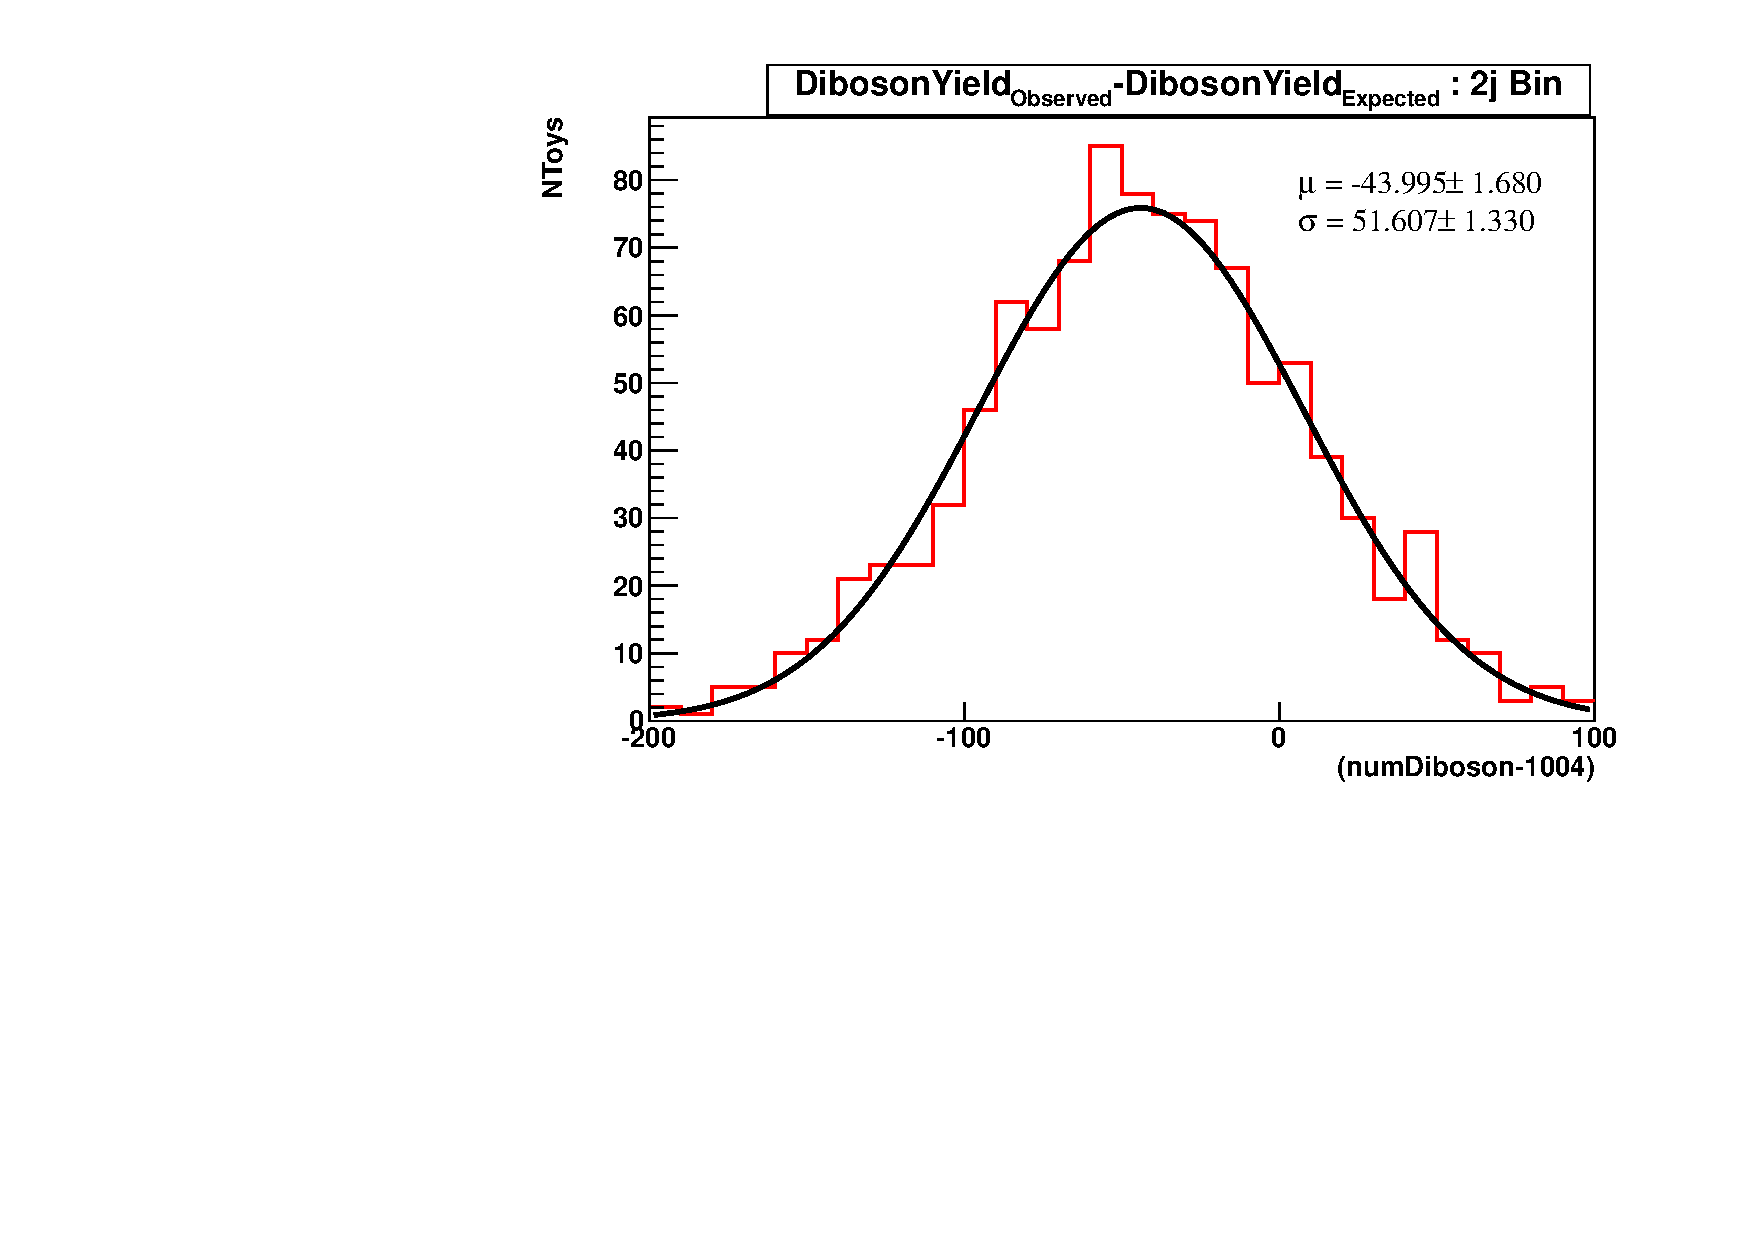
\includegraphics[width=0.48\textwidth]{figs/validation/ToyFits_DibosonYield_2j.pdf}
\put(-0.80,0.0){(a)} 
\unitlength=0.33\linewidth
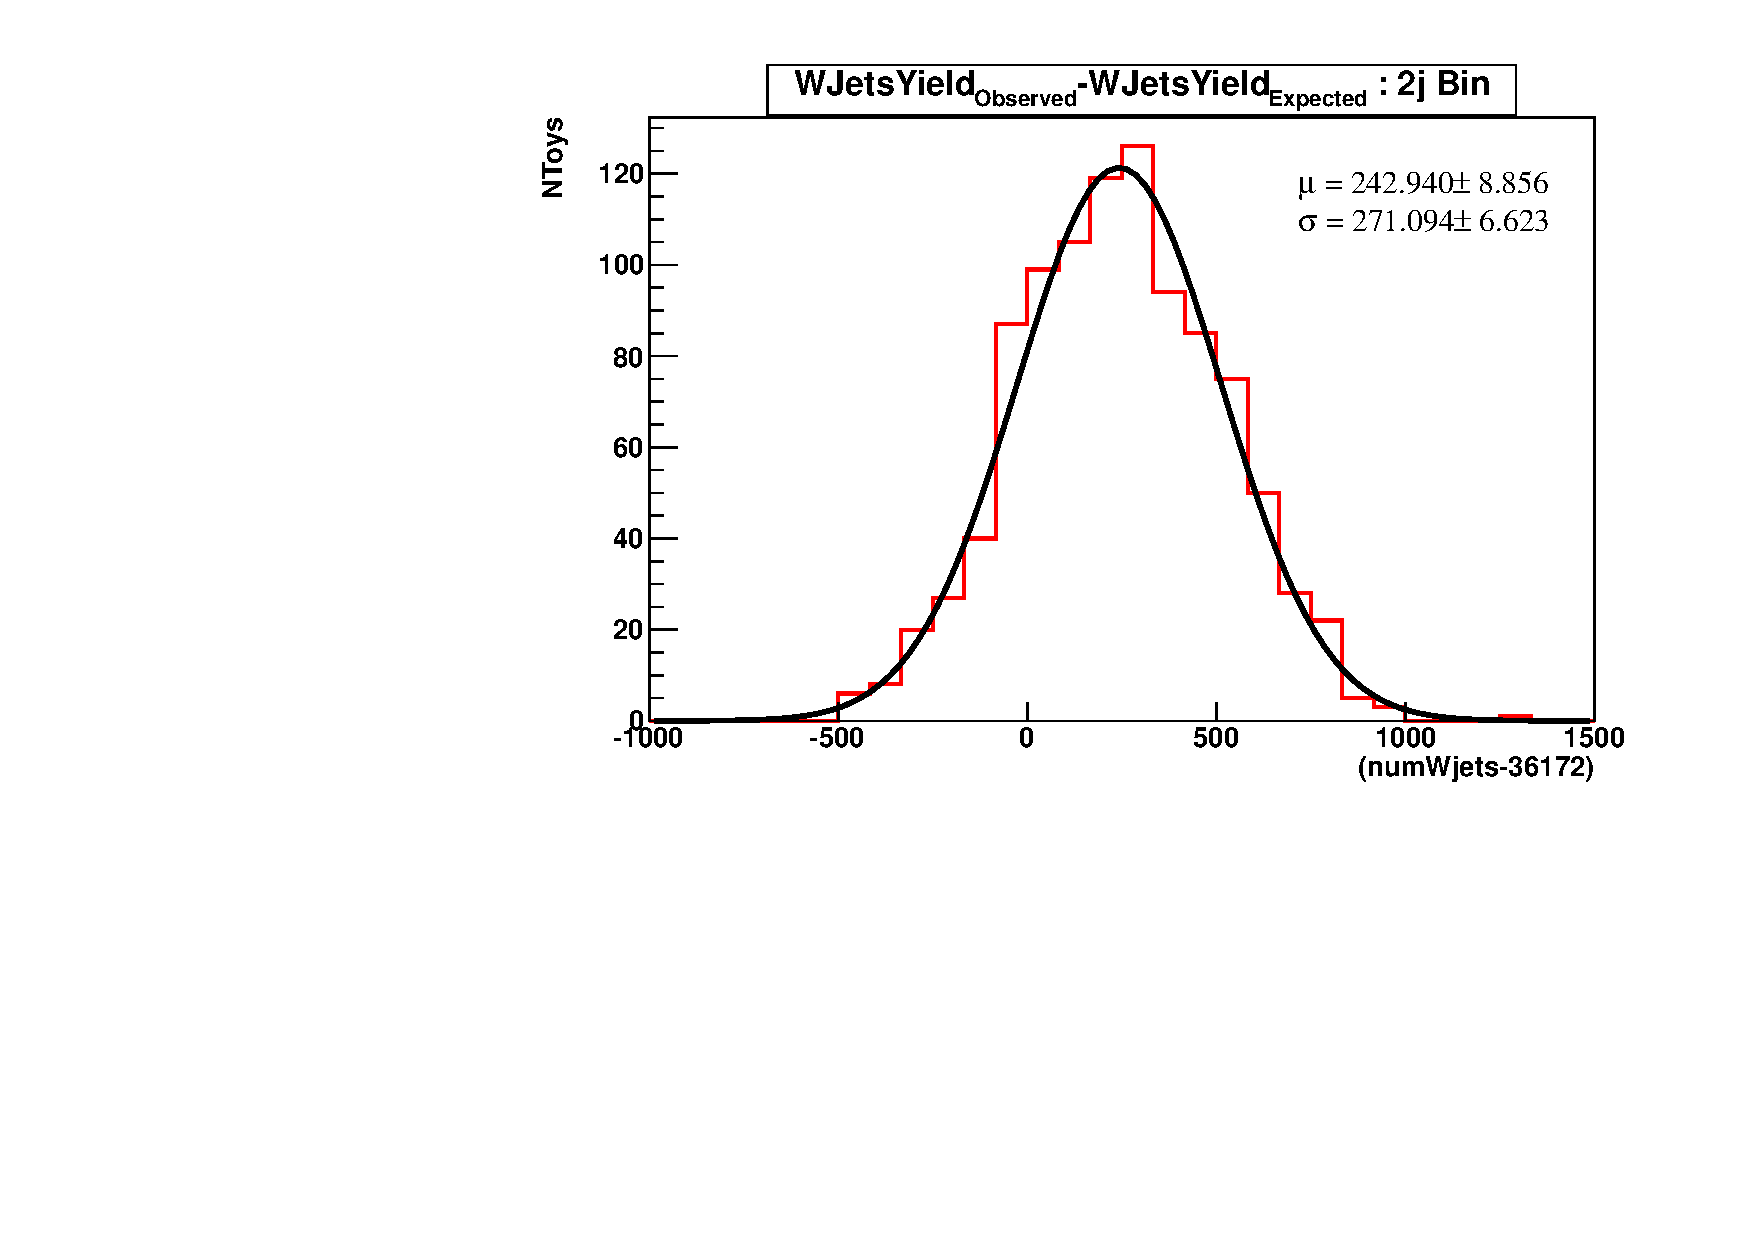
\includegraphics[width=0.48\textwidth]{figs/validation/ToyFits_WJetsYield_2j.pdf}
\put(-0.80,0.0){(b)} \\
\unitlength=0.33\linewidth
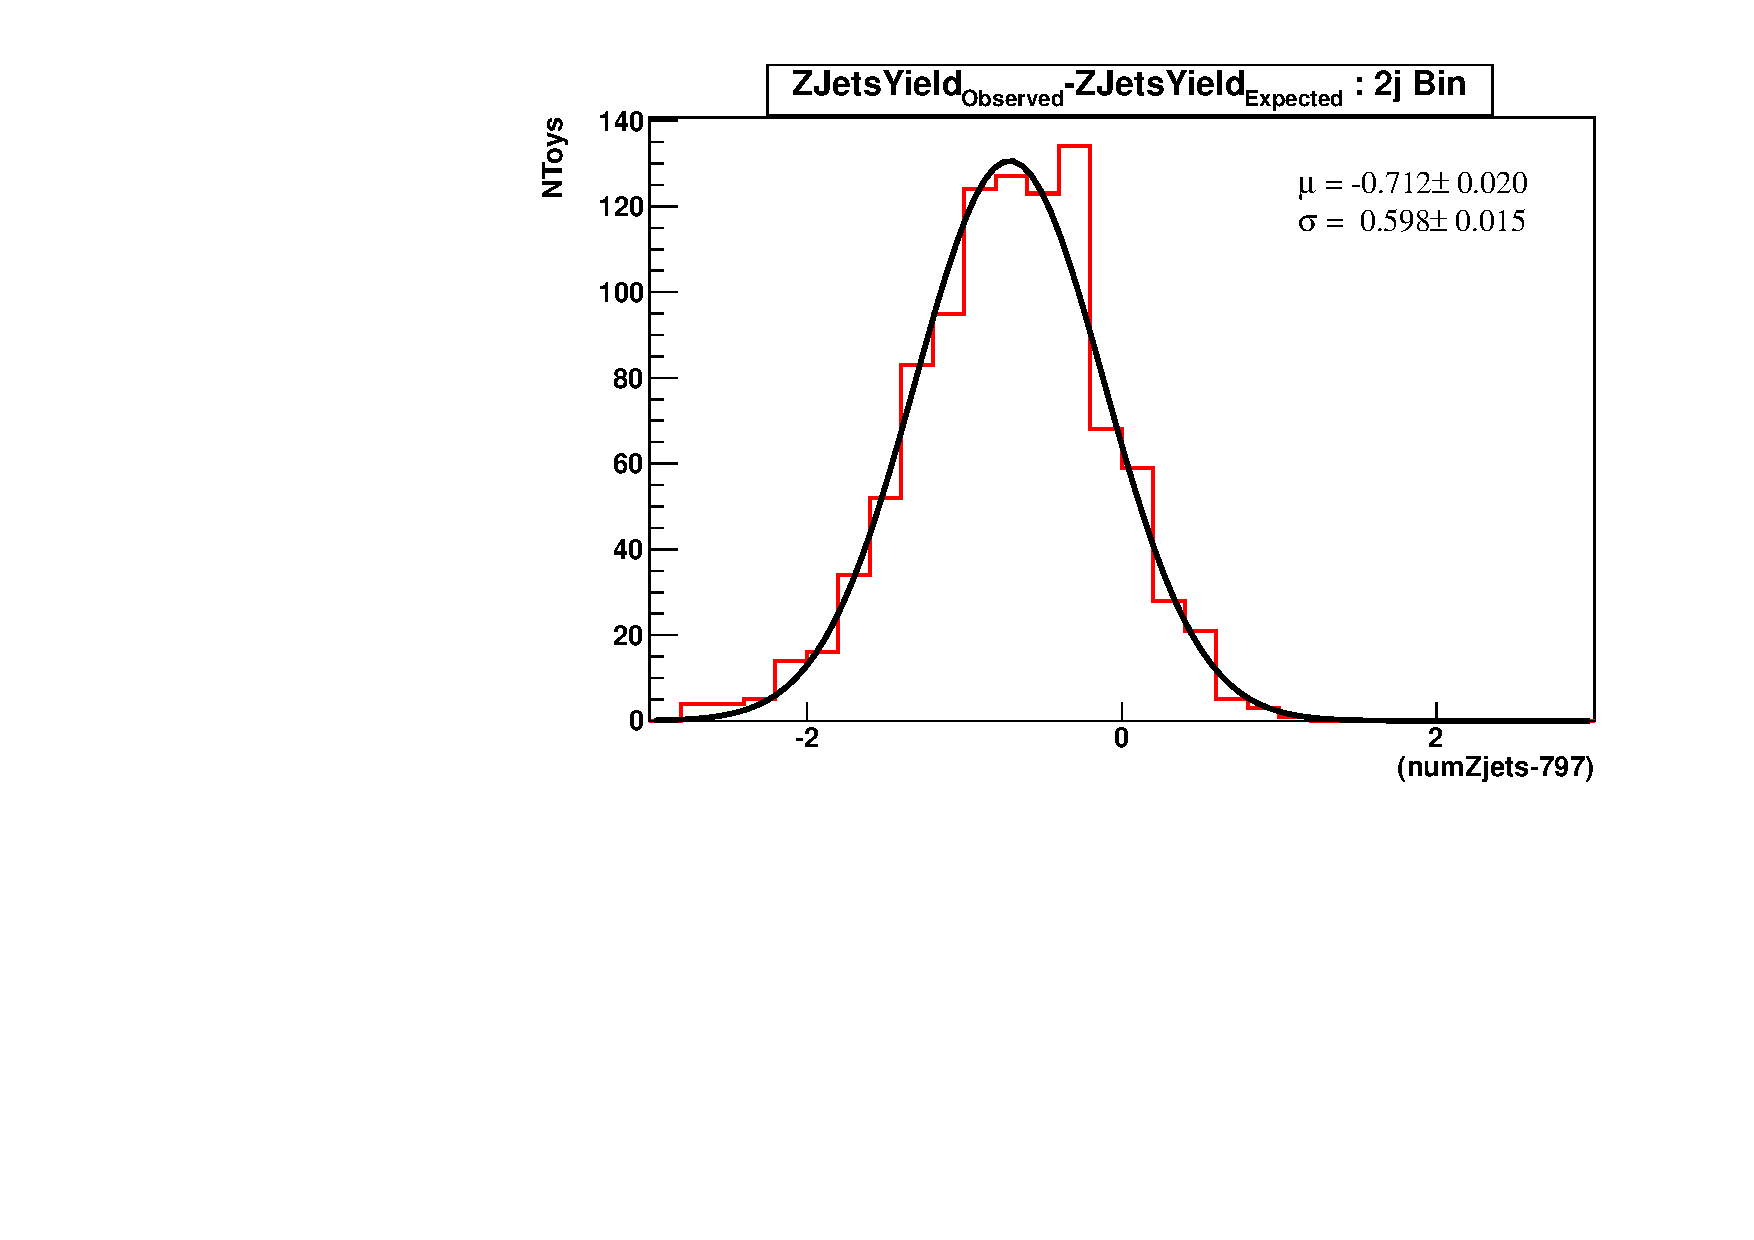
\includegraphics[width=0.48\textwidth]{figs/validation/ToyFits_ZJetsYield_2j.pdf}
\put(-0.80,0.0){(c)} 
\unitlength=0.33\linewidth
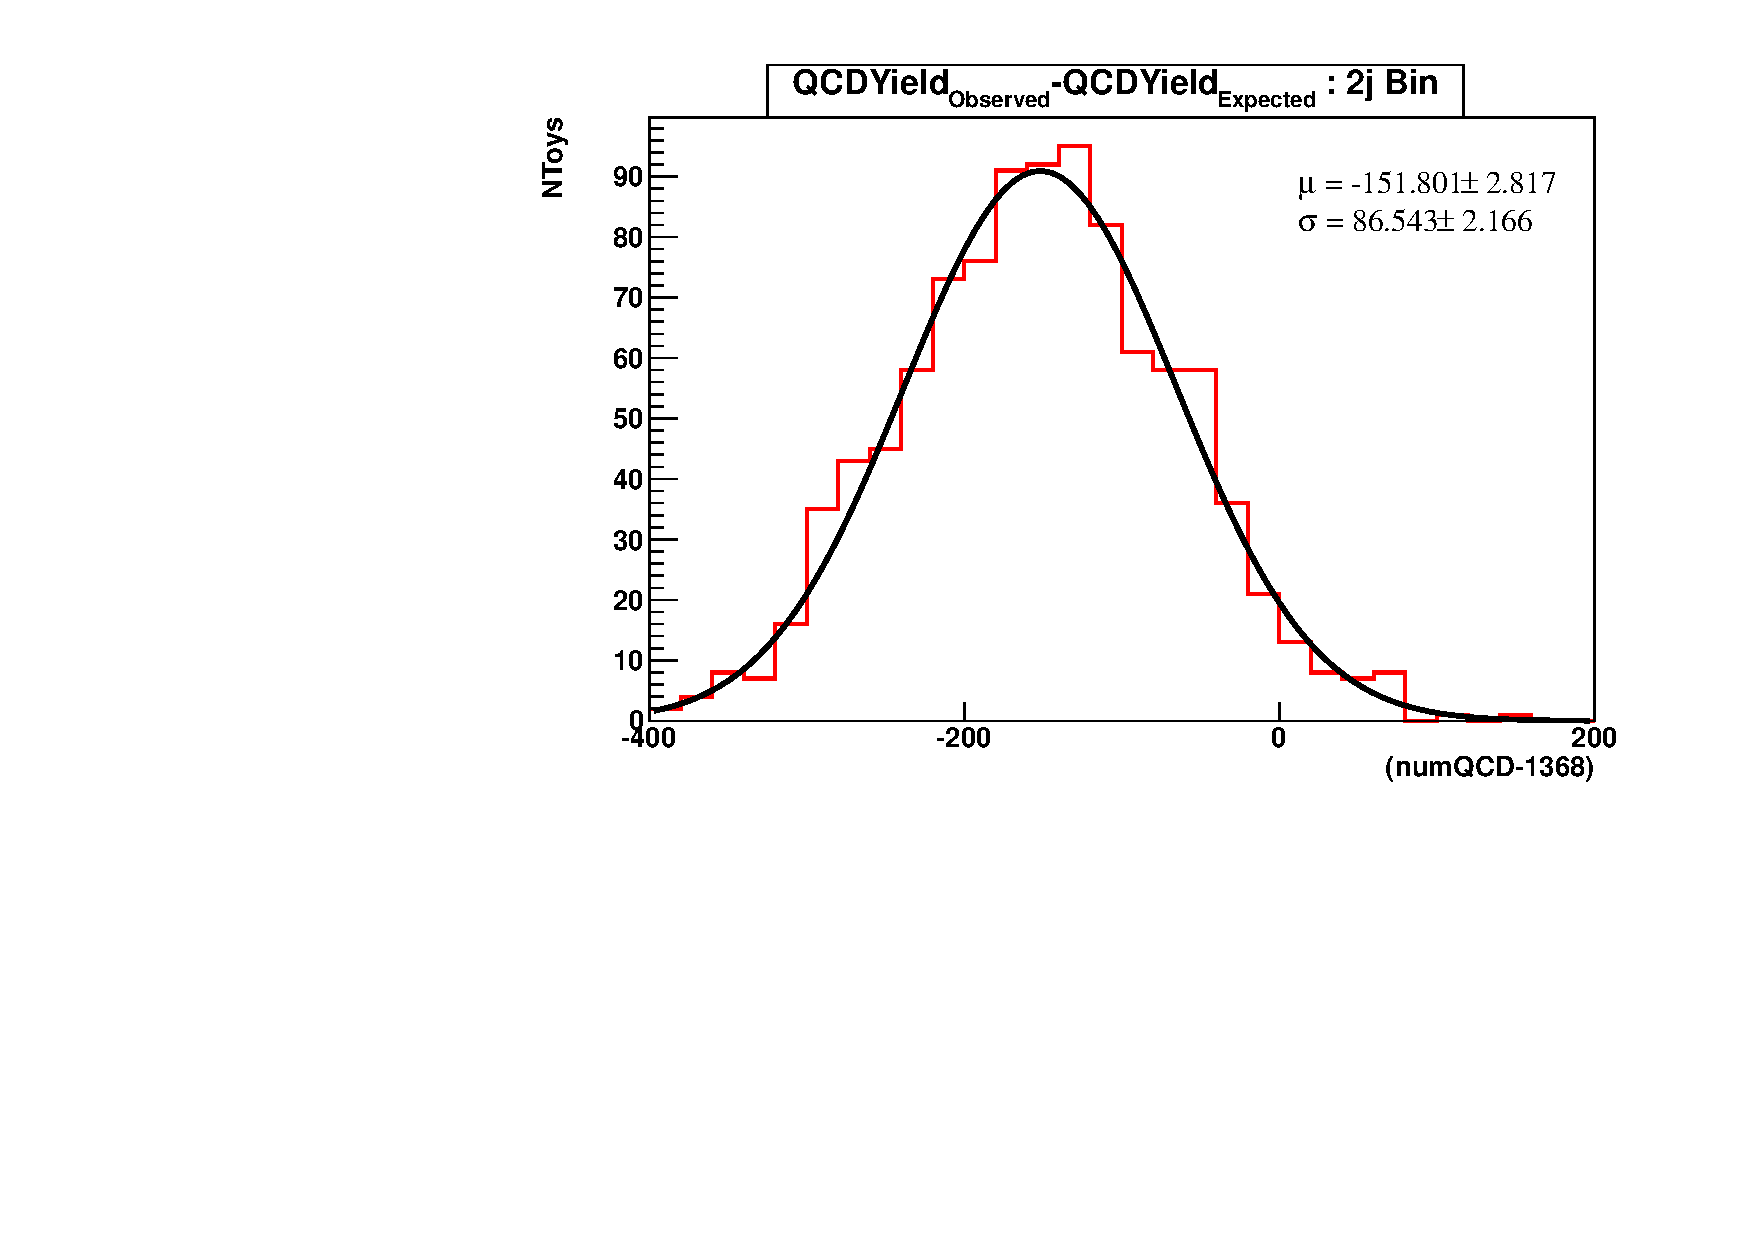
\includegraphics[width=0.48\textwidth]{figs/validation/ToyFits_QCDYield_2j.pdf}
\put(-0.80,0.0){(d)} \\
\unitlength=0.33\linewidth
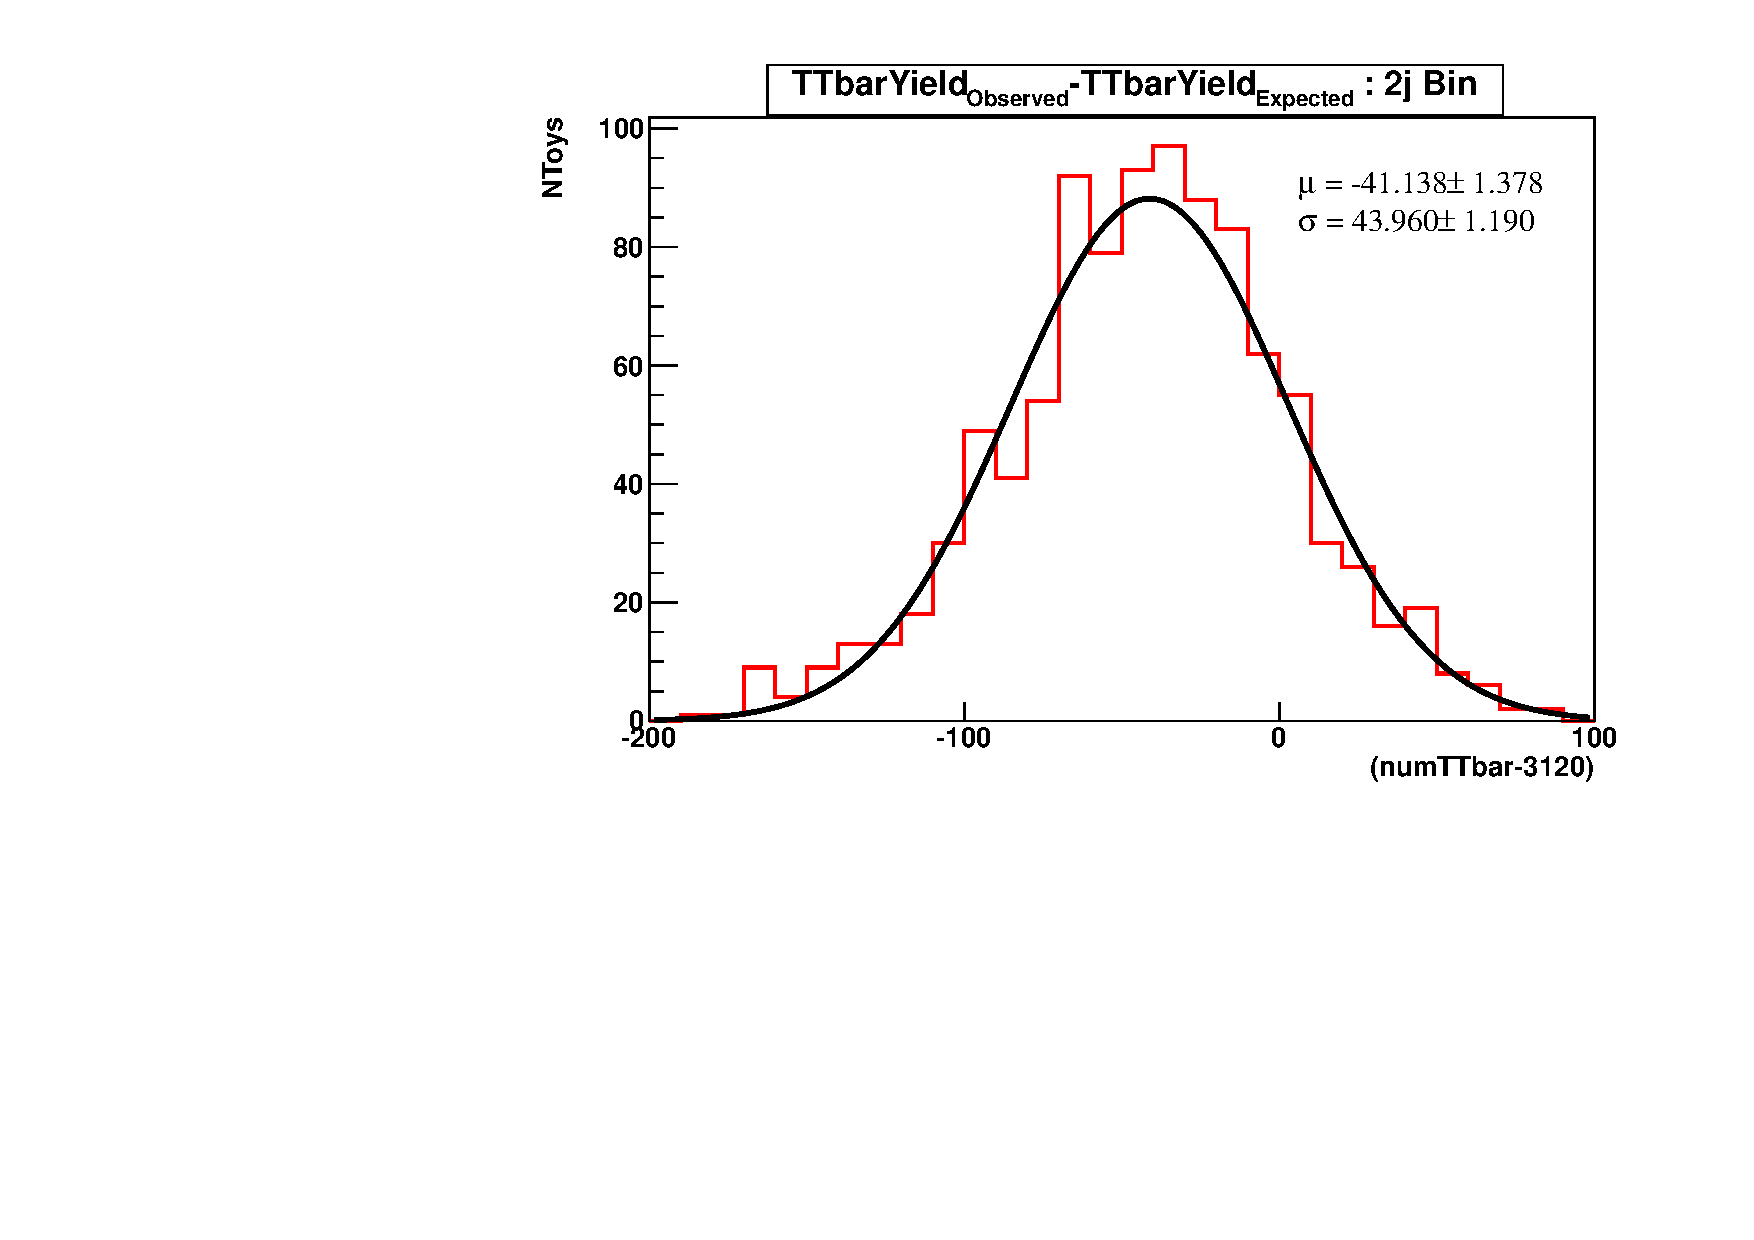
\includegraphics[width=0.48\textwidth]{figs/validation/ToyFits_TTbarYield_2j.pdf}
\put(-0.80,0.0){(e)} 
\unitlength=0.33\linewidth
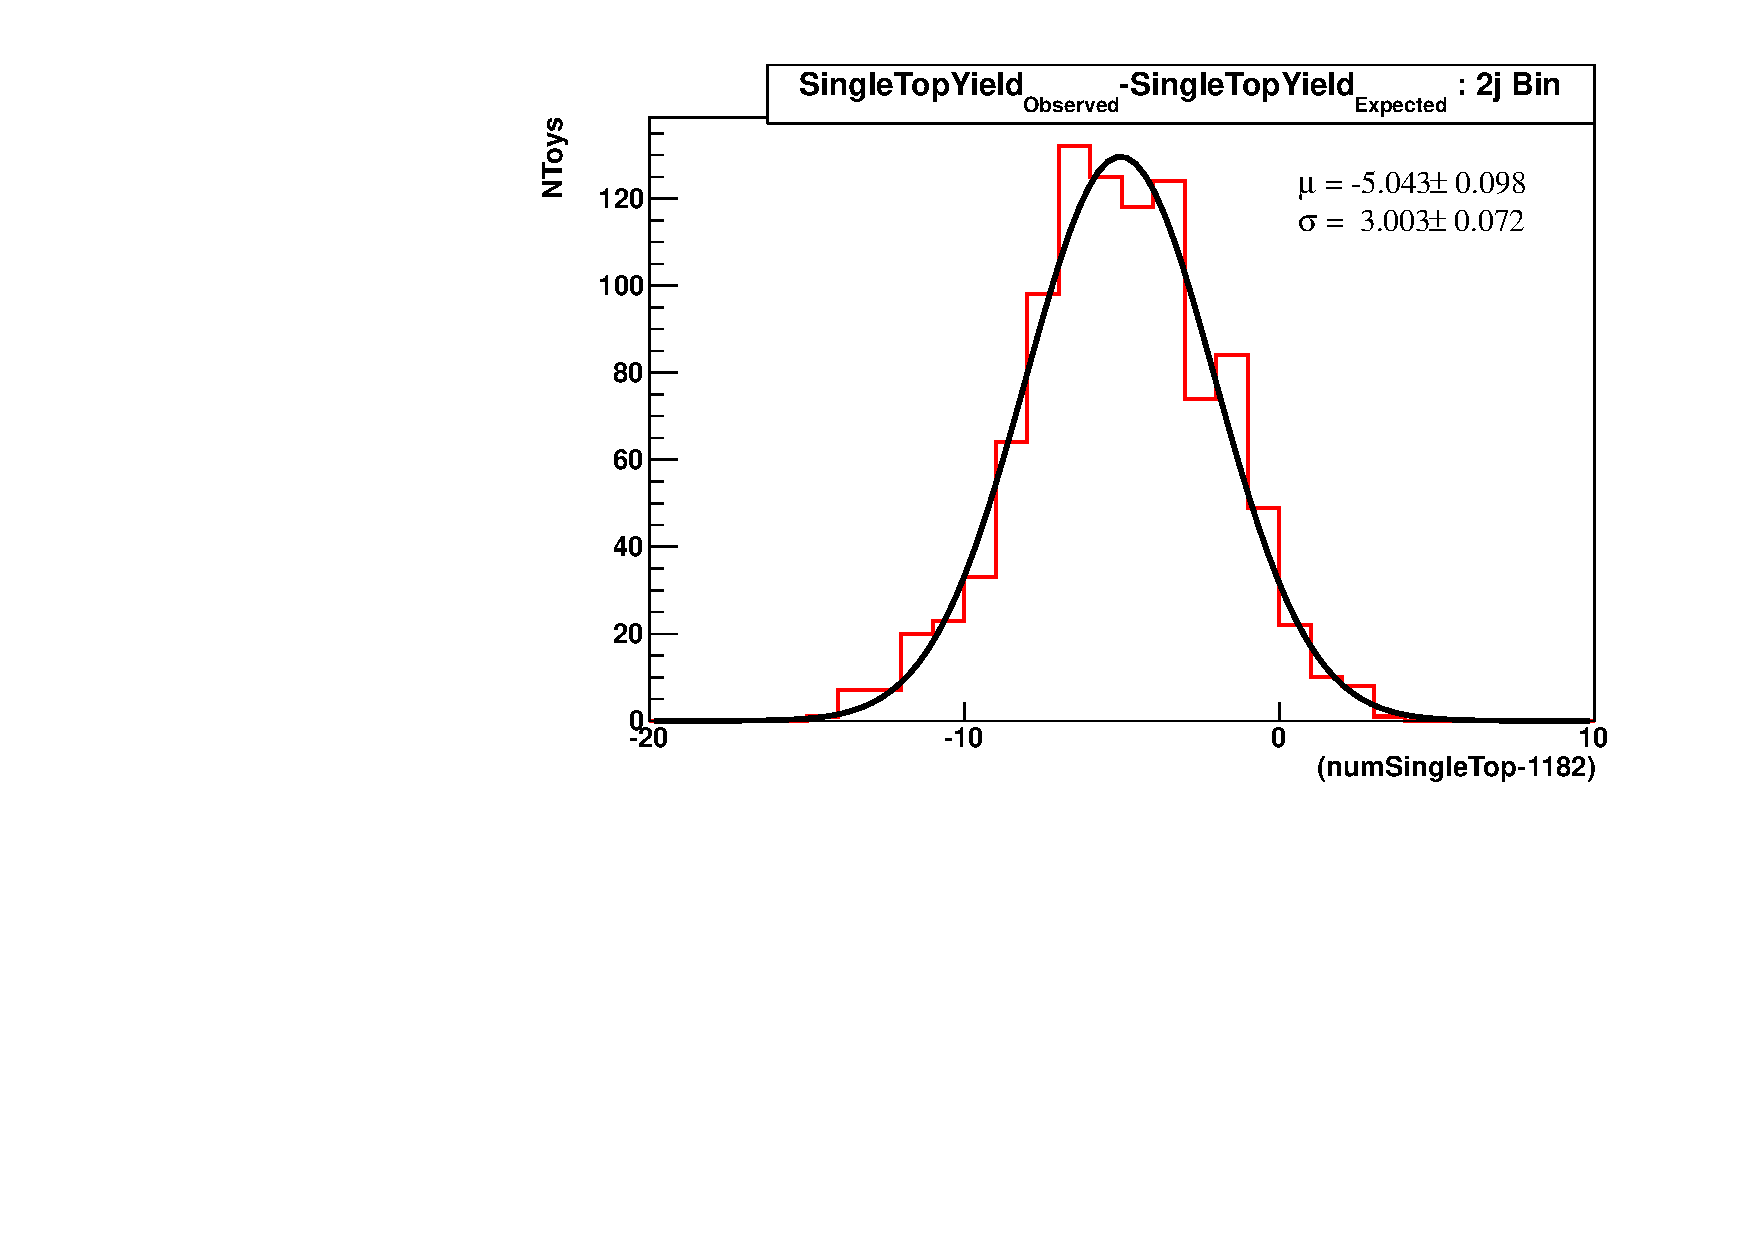
\includegraphics[width=0.48\textwidth]{figs/validation/ToyFits_SingleTopYield_2j.pdf}
\put(-0.80,0.0){(f)} 
\caption{Fit validation in the 2-jet bin using 1000 Toy MC datasets. Fitted-Expected yields for: (a) Diboson, (b) W+jets, (c) Z+jets, (d) QCD, (e) $t\bar{t}$, (f) Single top.} 
\label{fig:Validation_2j}}
\end{figure}
%%%%%%%
%%%%%%%
\begin{figure}[h!] {\centering
\unitlength=0.33\linewidth
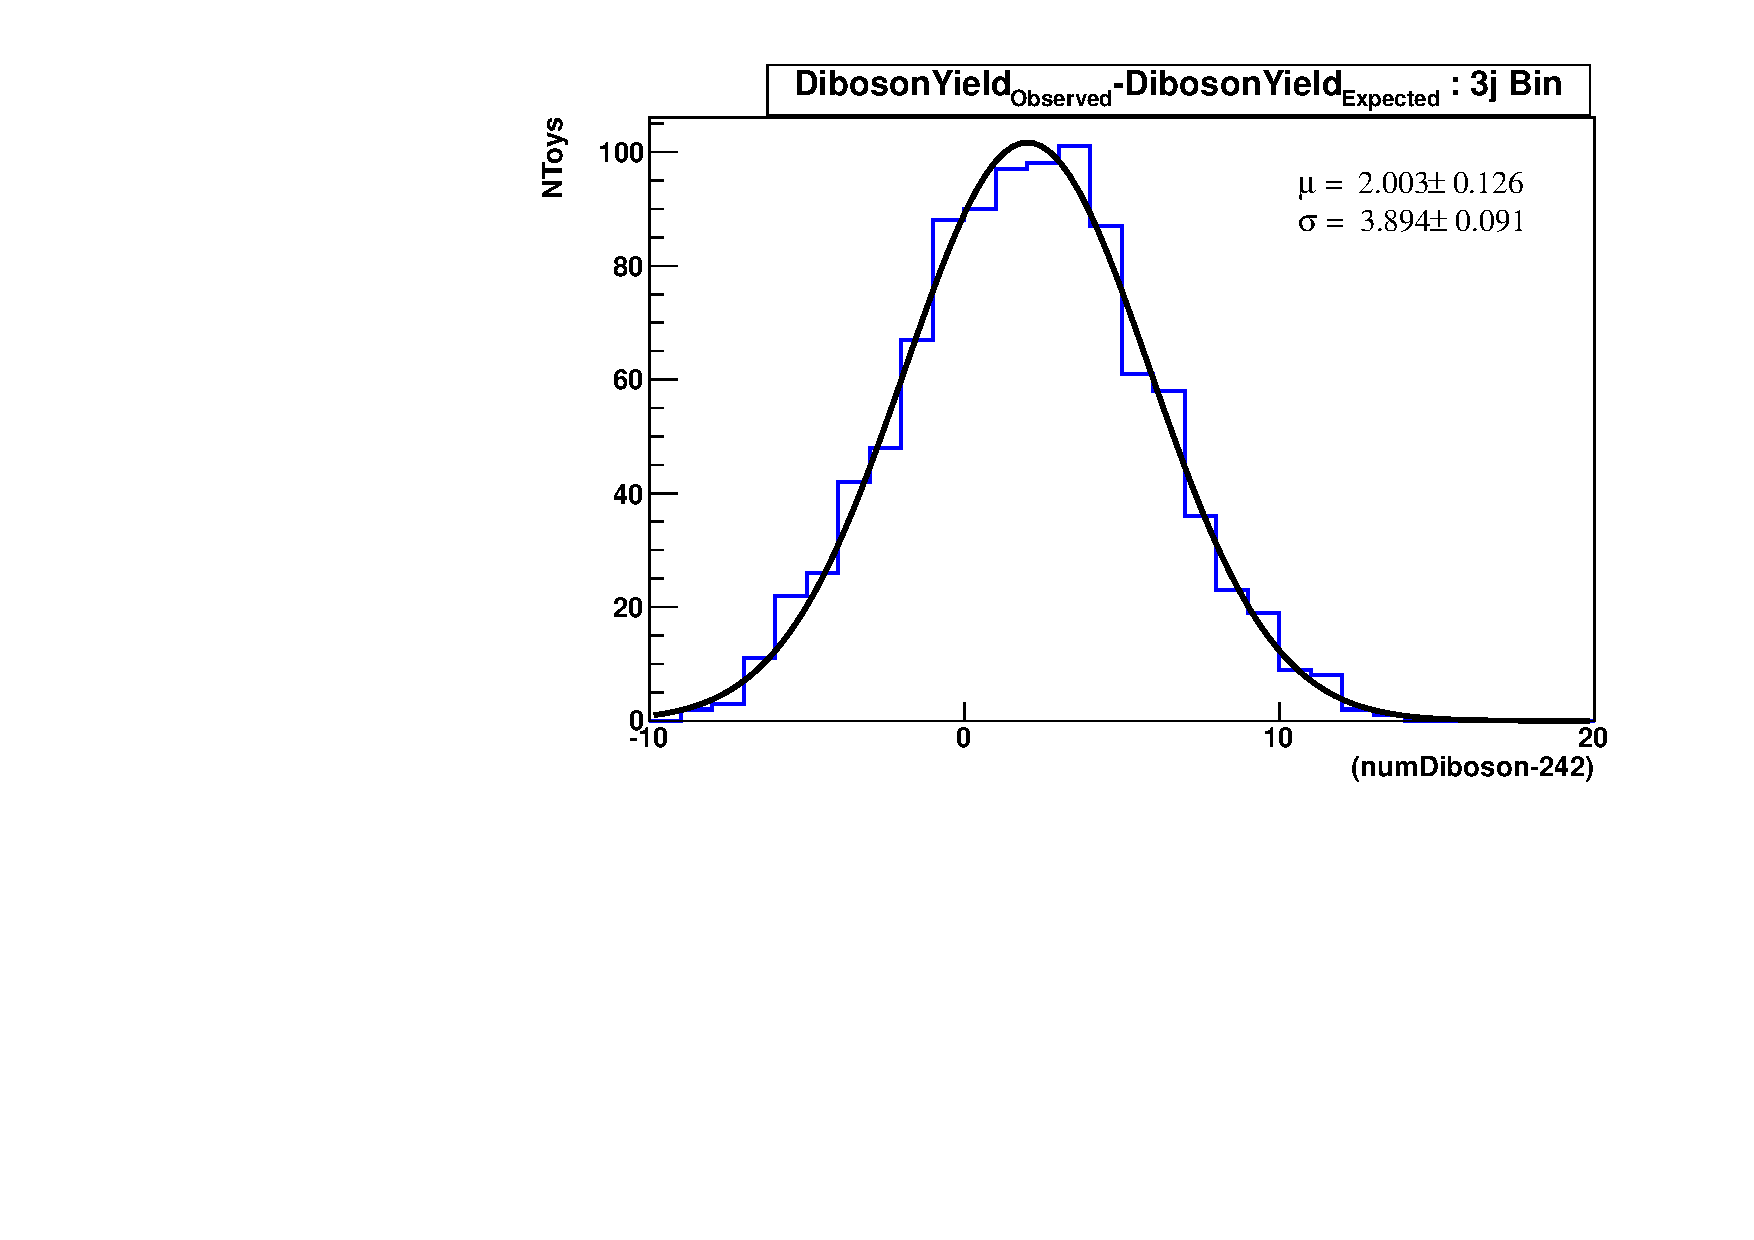
\includegraphics[width=0.48\textwidth]{figs/validation/ToyFits_DibosonYield_3j.pdf}
\put(-0.80,0.0){(a)} 
\unitlength=0.33\linewidth
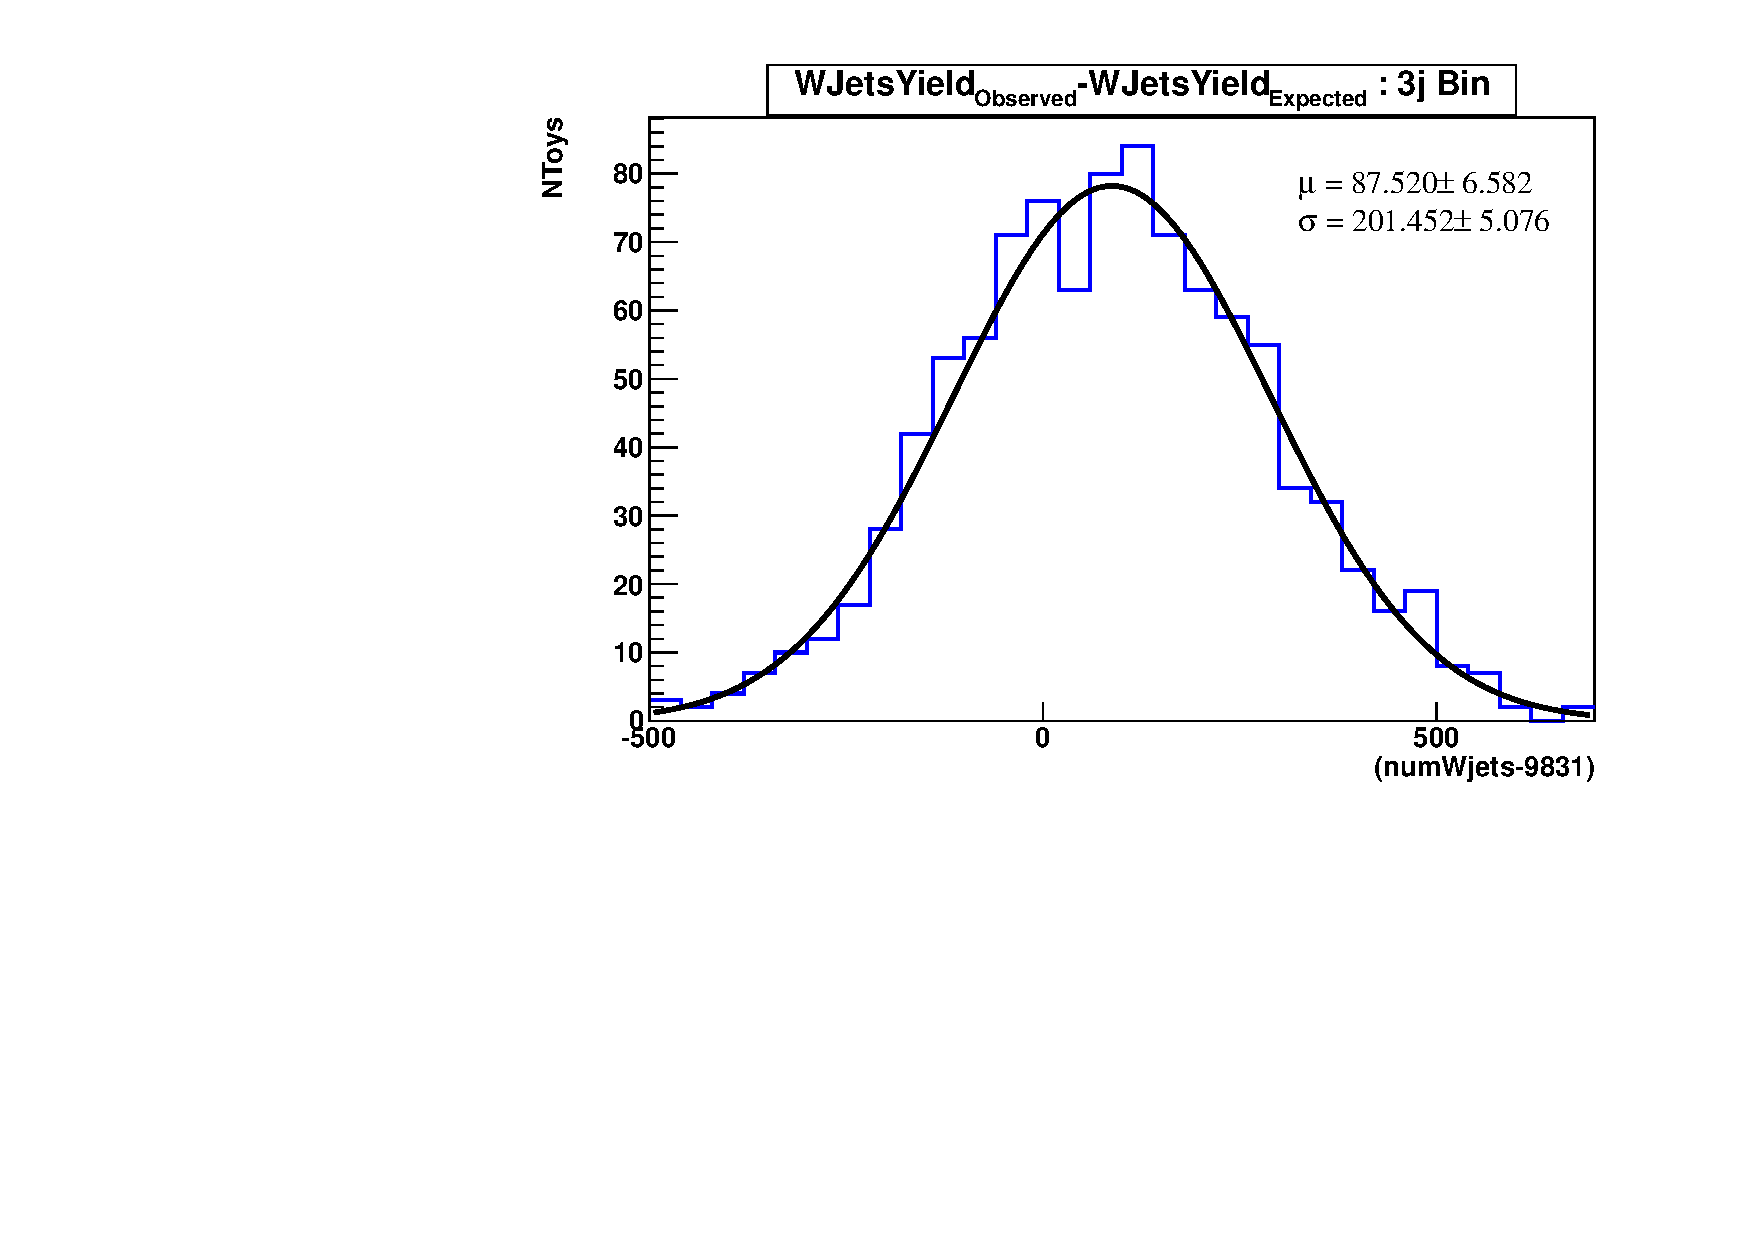
\includegraphics[width=0.48\textwidth]{figs/validation/ToyFits_WJetsYield_3j.pdf}
\put(-0.80,0.0){(b)} \\
\unitlength=0.33\linewidth
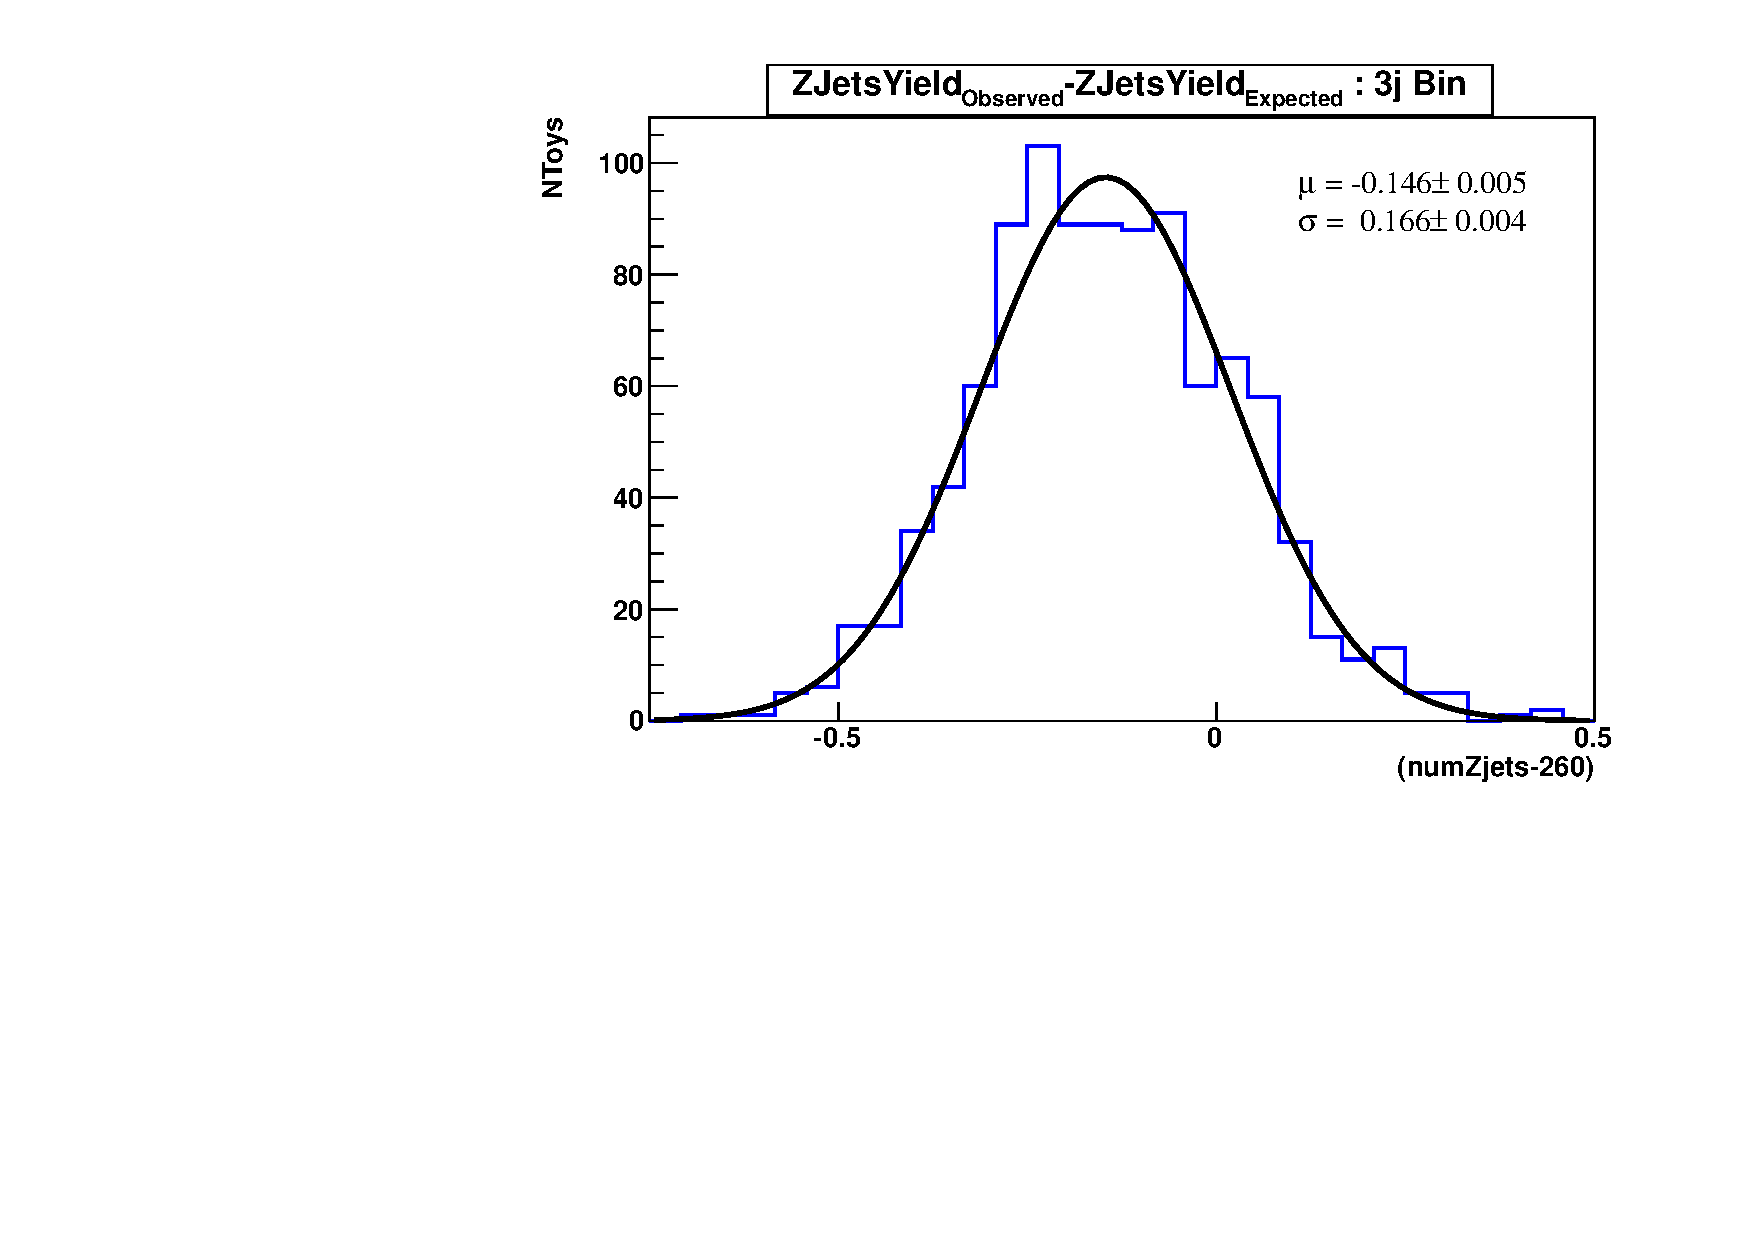
\includegraphics[width=0.48\textwidth]{figs/validation/ToyFits_ZJetsYield_3j.pdf}
\put(-0.80,0.0){(c)} 
\unitlength=0.33\linewidth
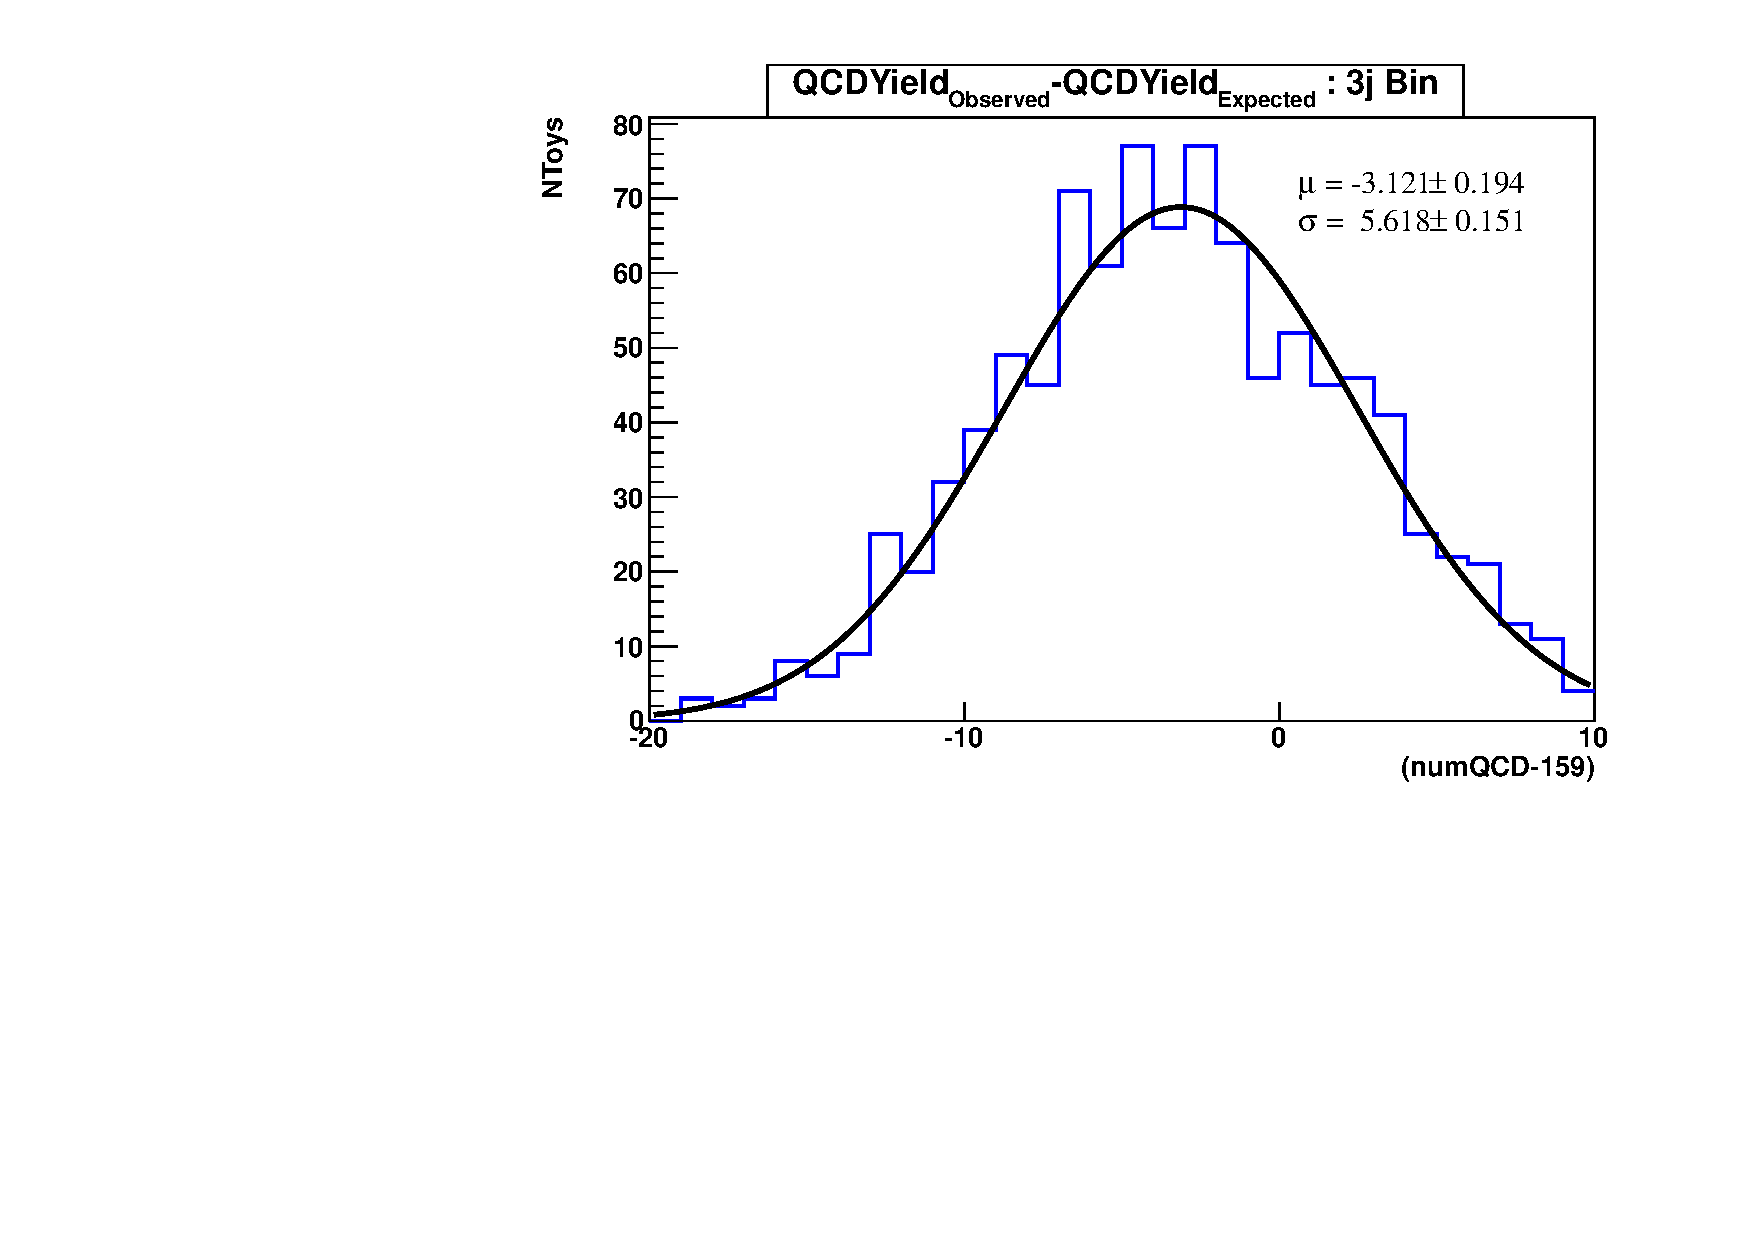
\includegraphics[width=0.48\textwidth]{figs/validation/ToyFits_QCDYield_3j.pdf}
\put(-0.80,0.0){(d)} \\
\unitlength=0.33\linewidth
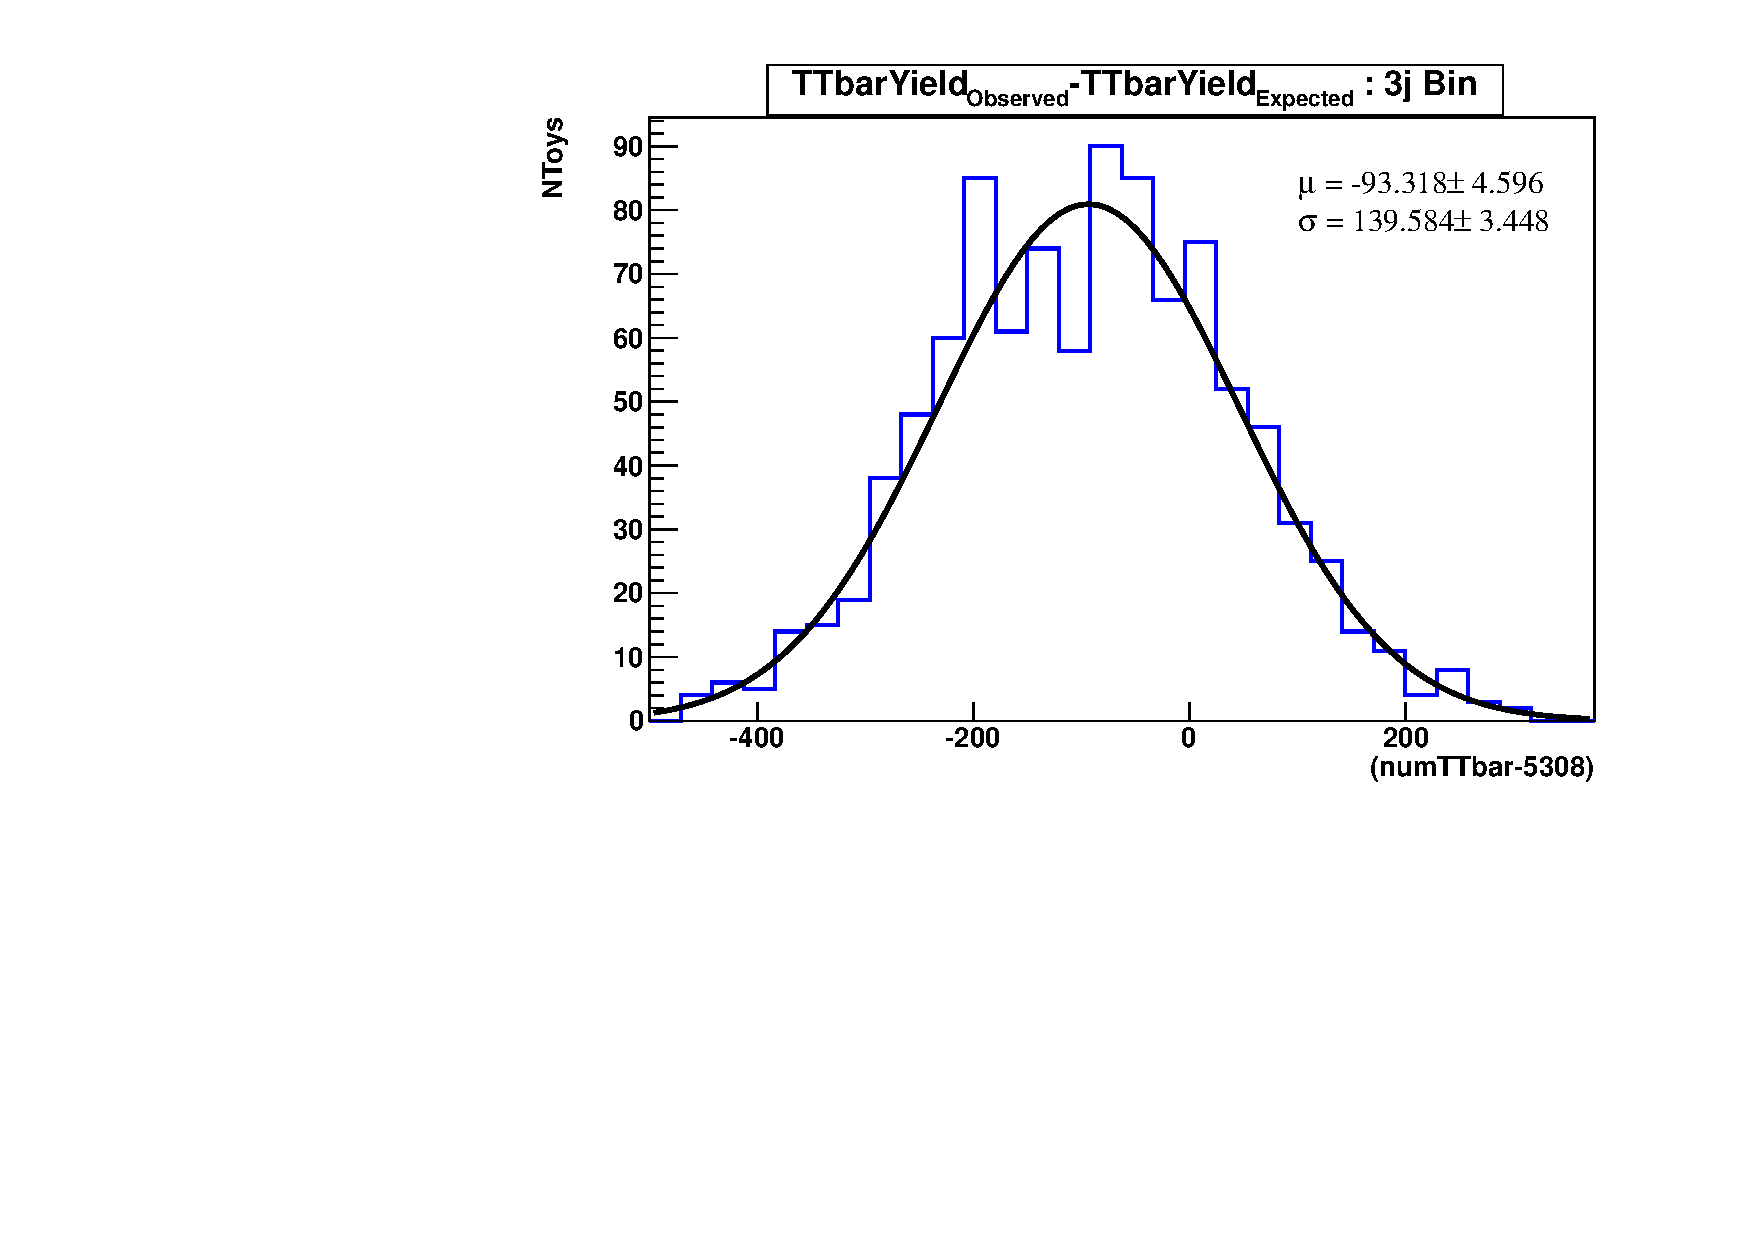
\includegraphics[width=0.48\textwidth]{figs/validation/ToyFits_TTbarYield_3j.pdf}
\put(-0.80,0.0){(e)} 
\unitlength=0.33\linewidth
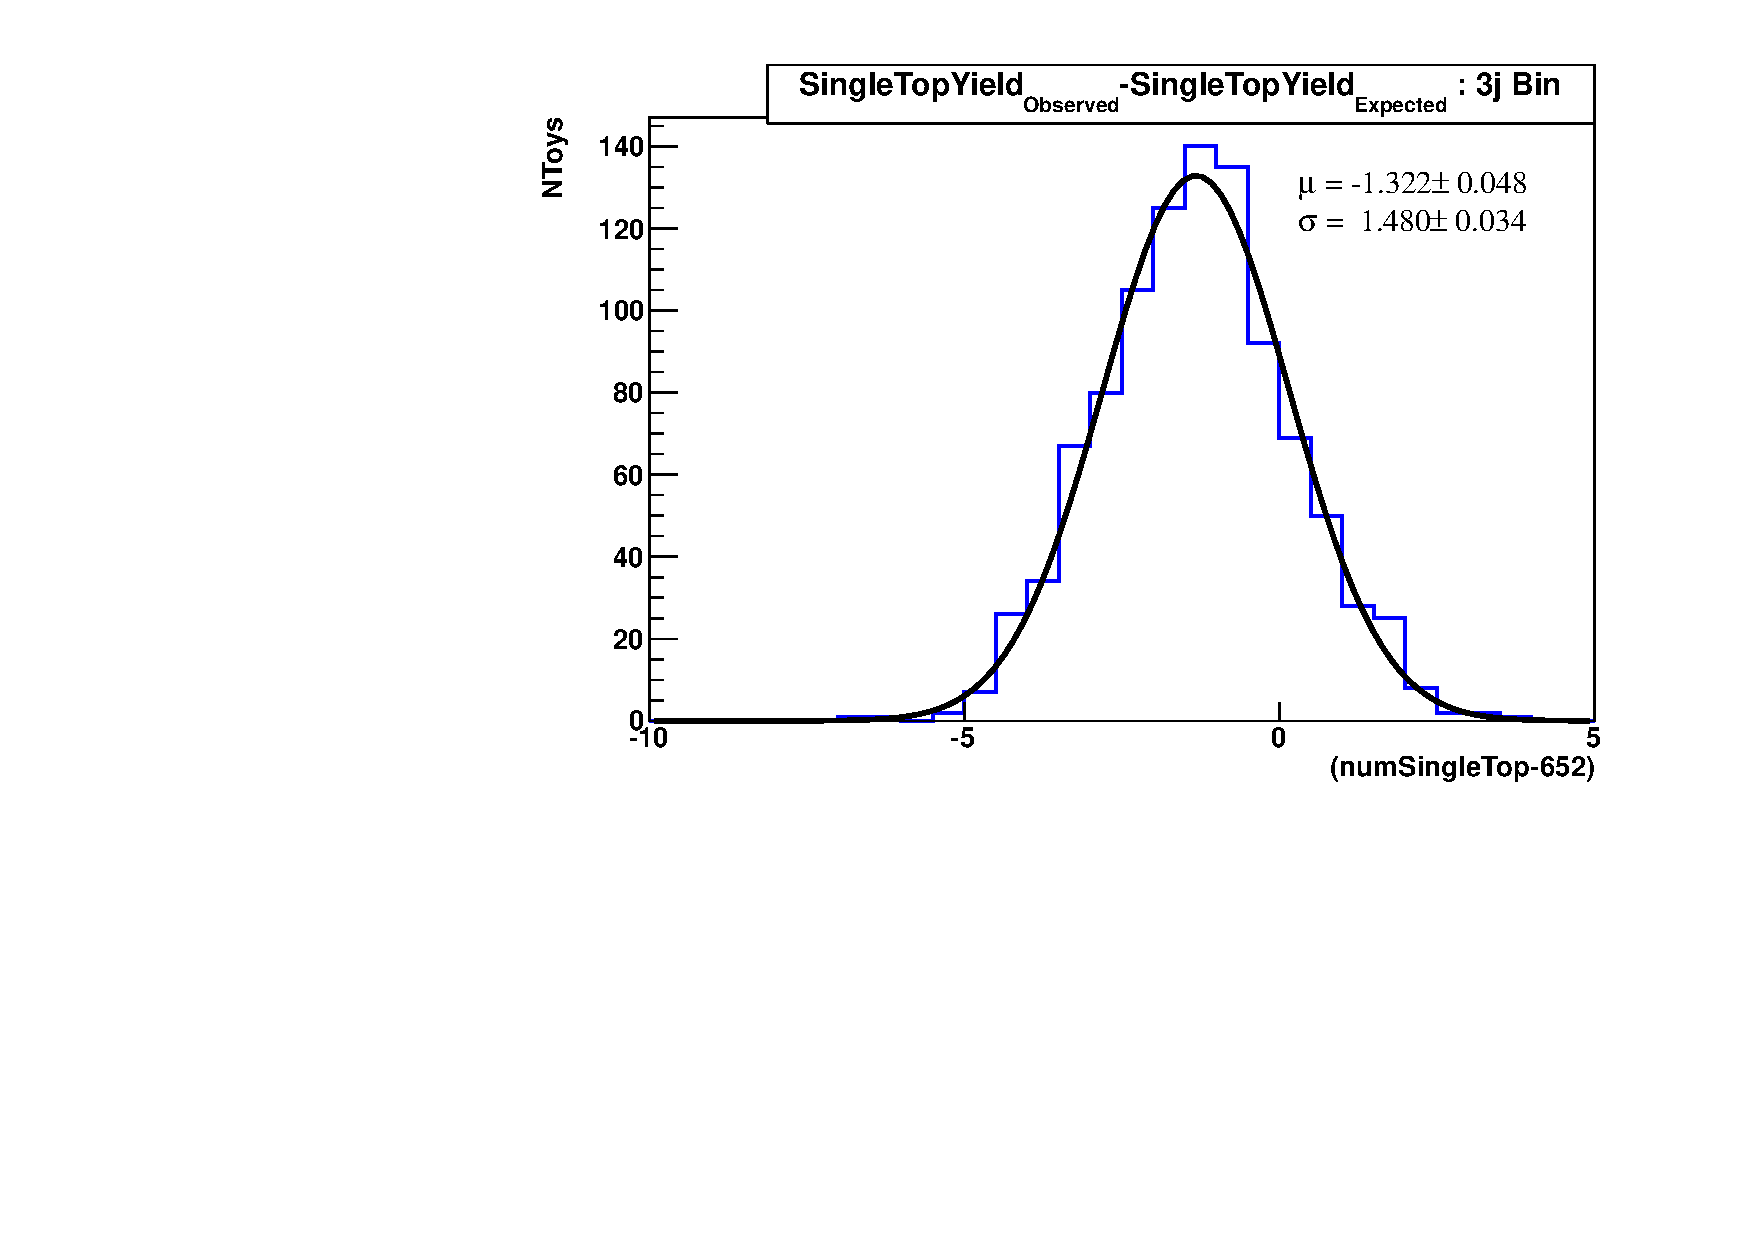
\includegraphics[width=0.48\textwidth]{figs/validation/ToyFits_SingleTopYield_3j.pdf}
\put(-0.80,0.0){(f)} 
\caption{Fit validation in the 3-jet bin using 1000 Toy MC datasets. Fitted-Expected yields for: (a) Diboson, (b) W+jets, (c) Z+jets, (d) QCD, (e) $t\bar{t}$, (f) Single top.} 
\label{fig:Validation_3j}}
\end{figure}
%%%%%%%
%%%%%%%
\begin{figure}[h!] {\centering
\unitlength=0.33\linewidth
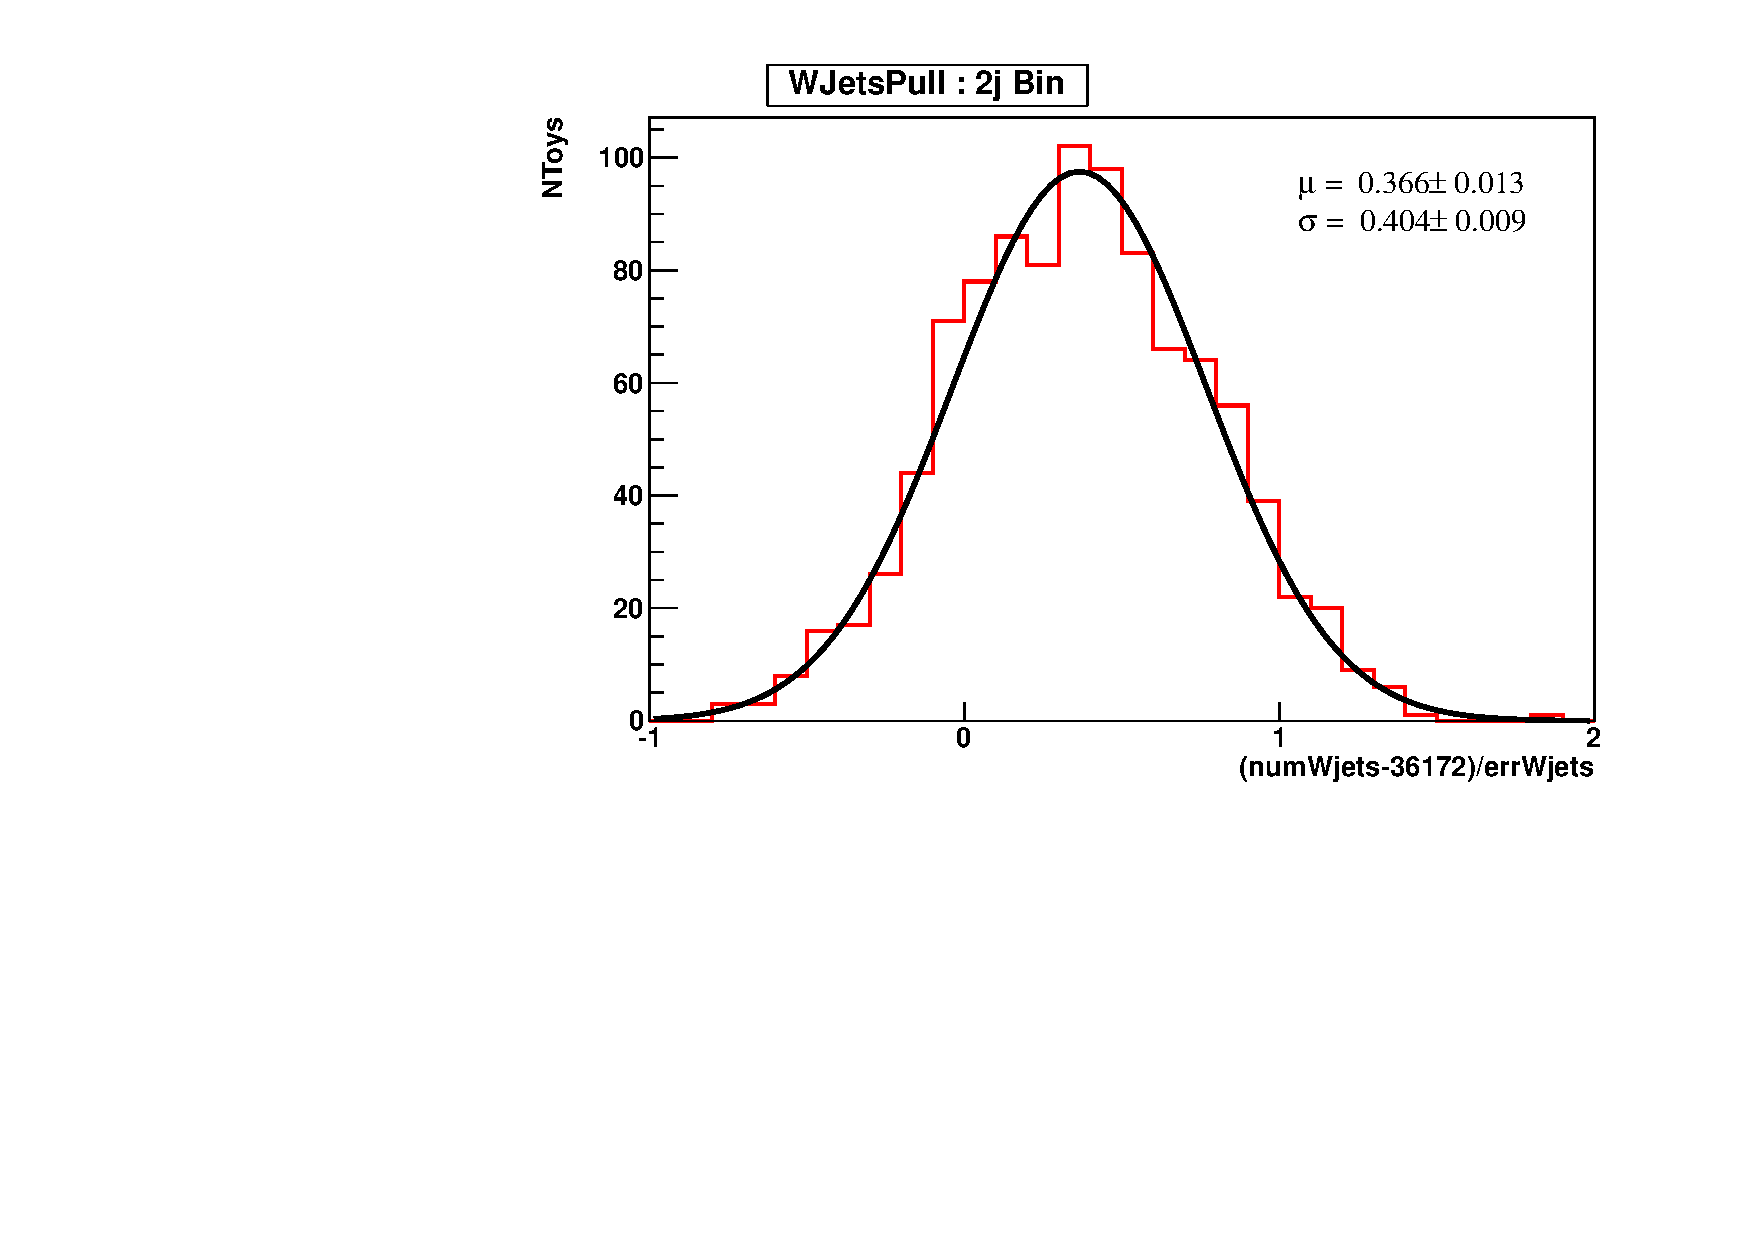
\includegraphics[width=0.48\textwidth]{figs/validation/ToyFits_WJetsPull_2j.pdf}
\put(-0.80,0.0){(a)} 
\unitlength=0.33\linewidth
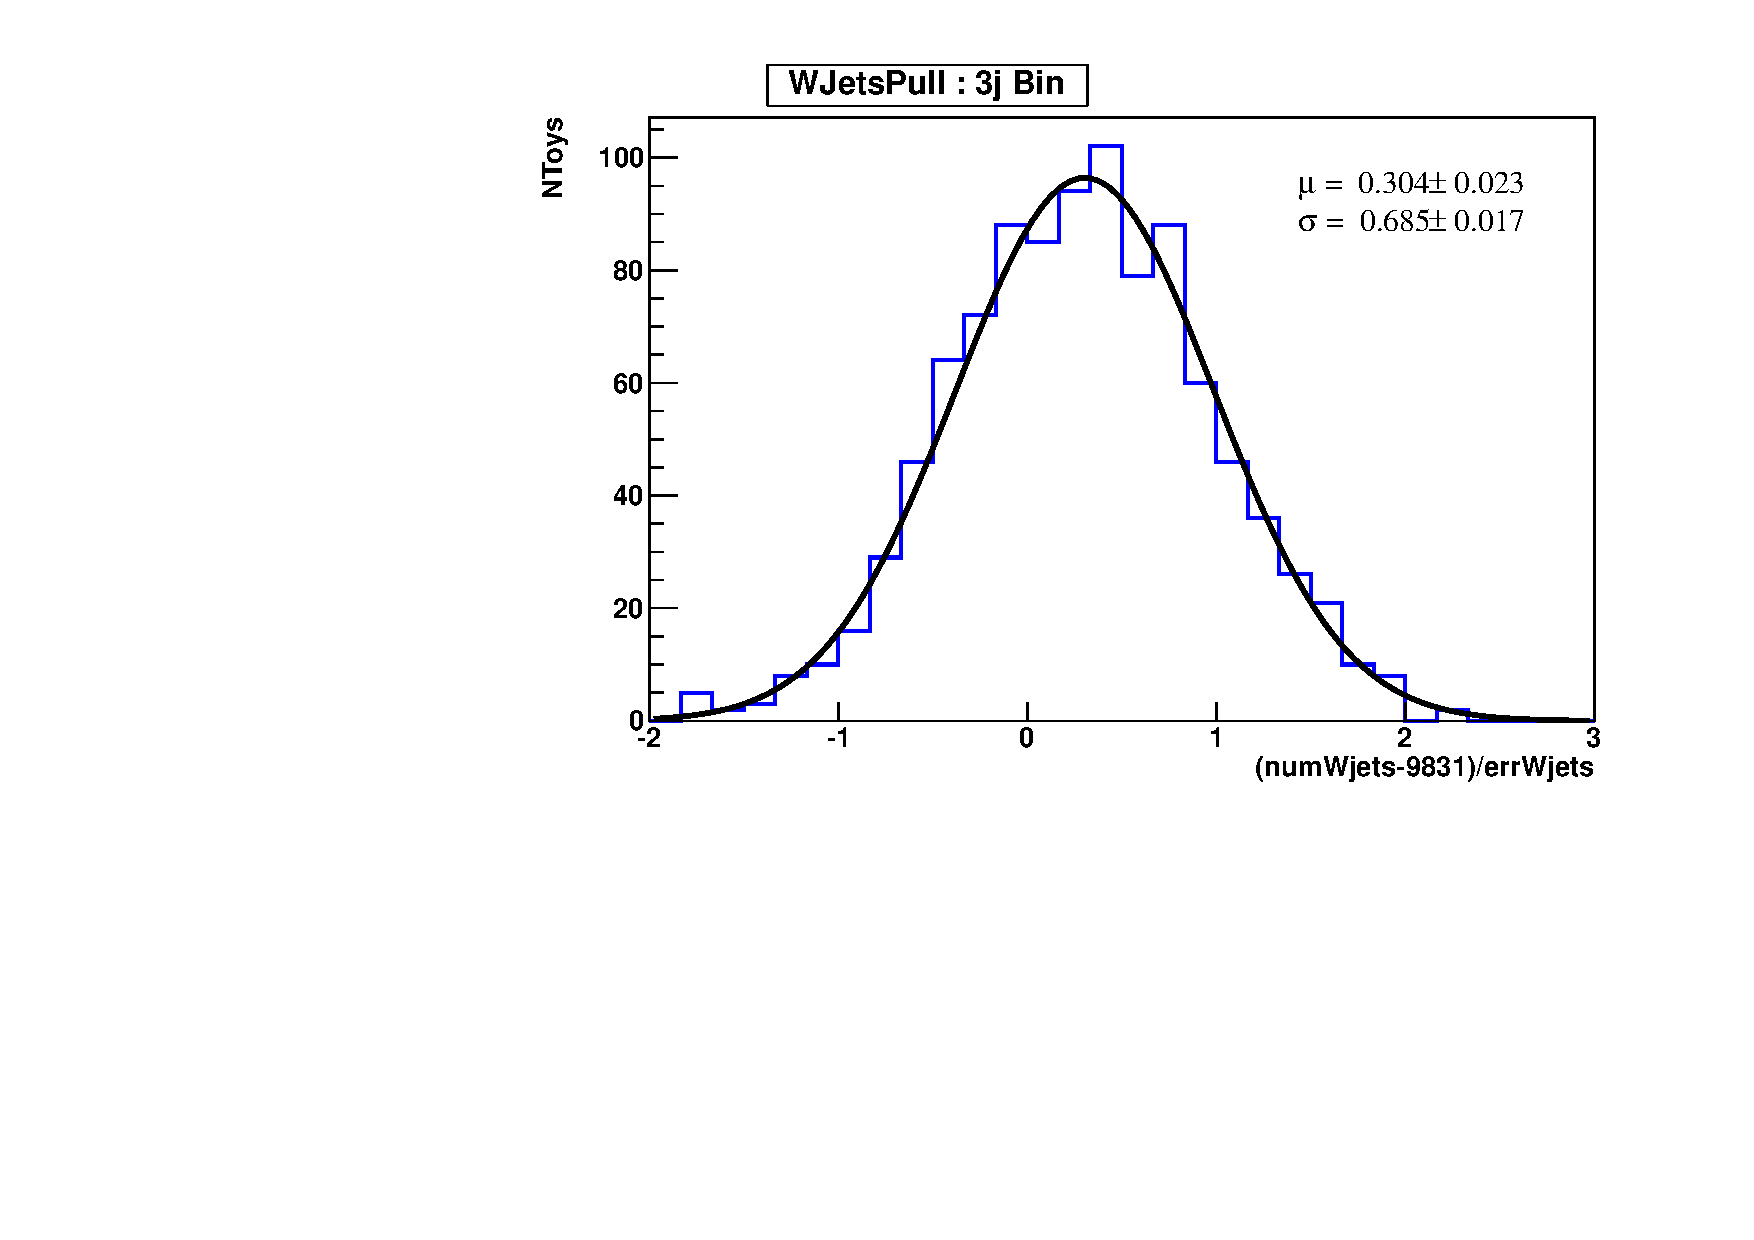
\includegraphics[width=0.48\textwidth]{figs/validation/ToyFits_WJetsPull_3j.pdf}
\put(-0.80,0.0){(b)}
\caption{Fit validation using 1000 Toy MC datasets. W+jets Pulls=(Observed-Expected)/Error for (a) 2 Jet Bit and (b) 3 Jet bin.}
\label{fig:Validation_PullsWjj}}
\end{figure}
%%%%%%%
%%%%%%%
\begin{figure}[h!] {\centering
\unitlength=0.33\linewidth
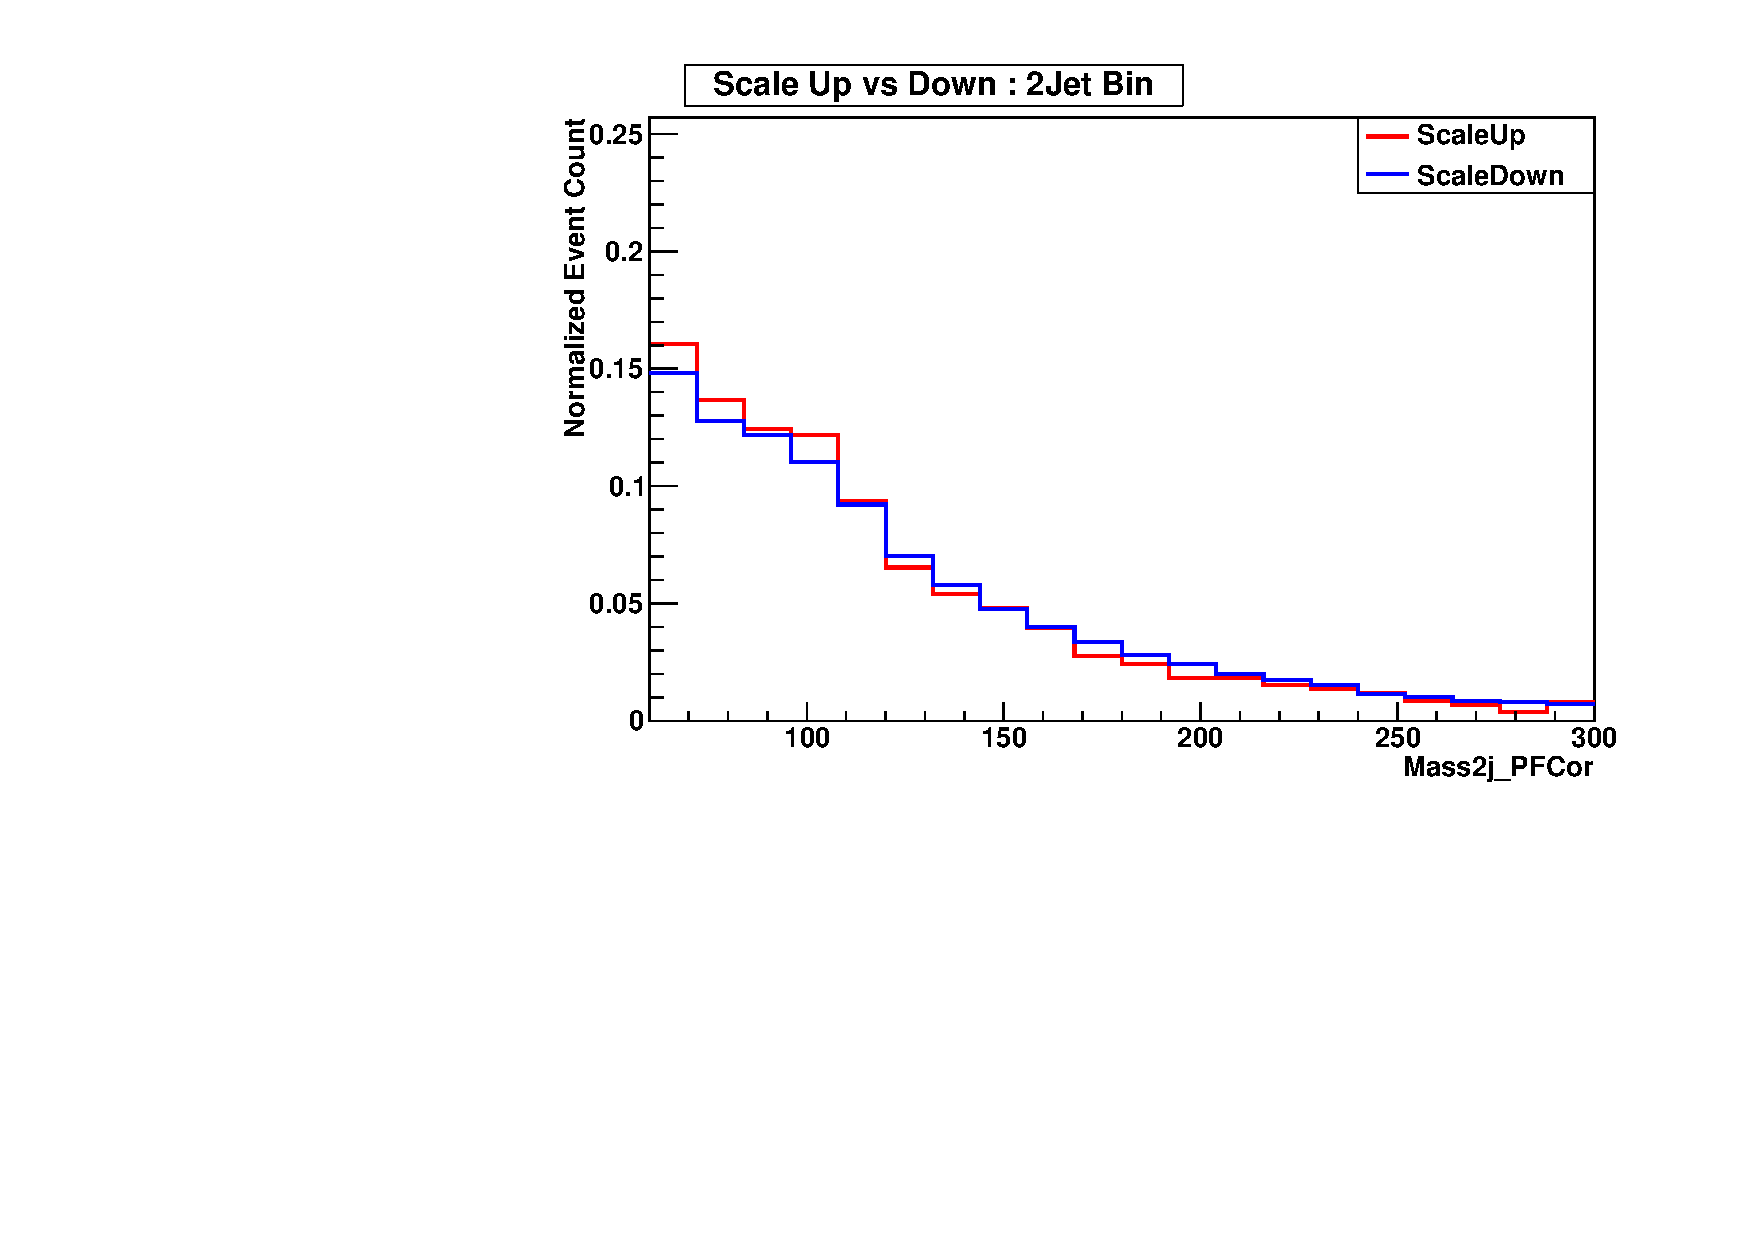
\includegraphics[width=0.48\textwidth]{figs/validation/ShapeComp_Scale2j.pdf}
\put(-0.80,0.0){(a)} 
\unitlength=0.33\linewidth
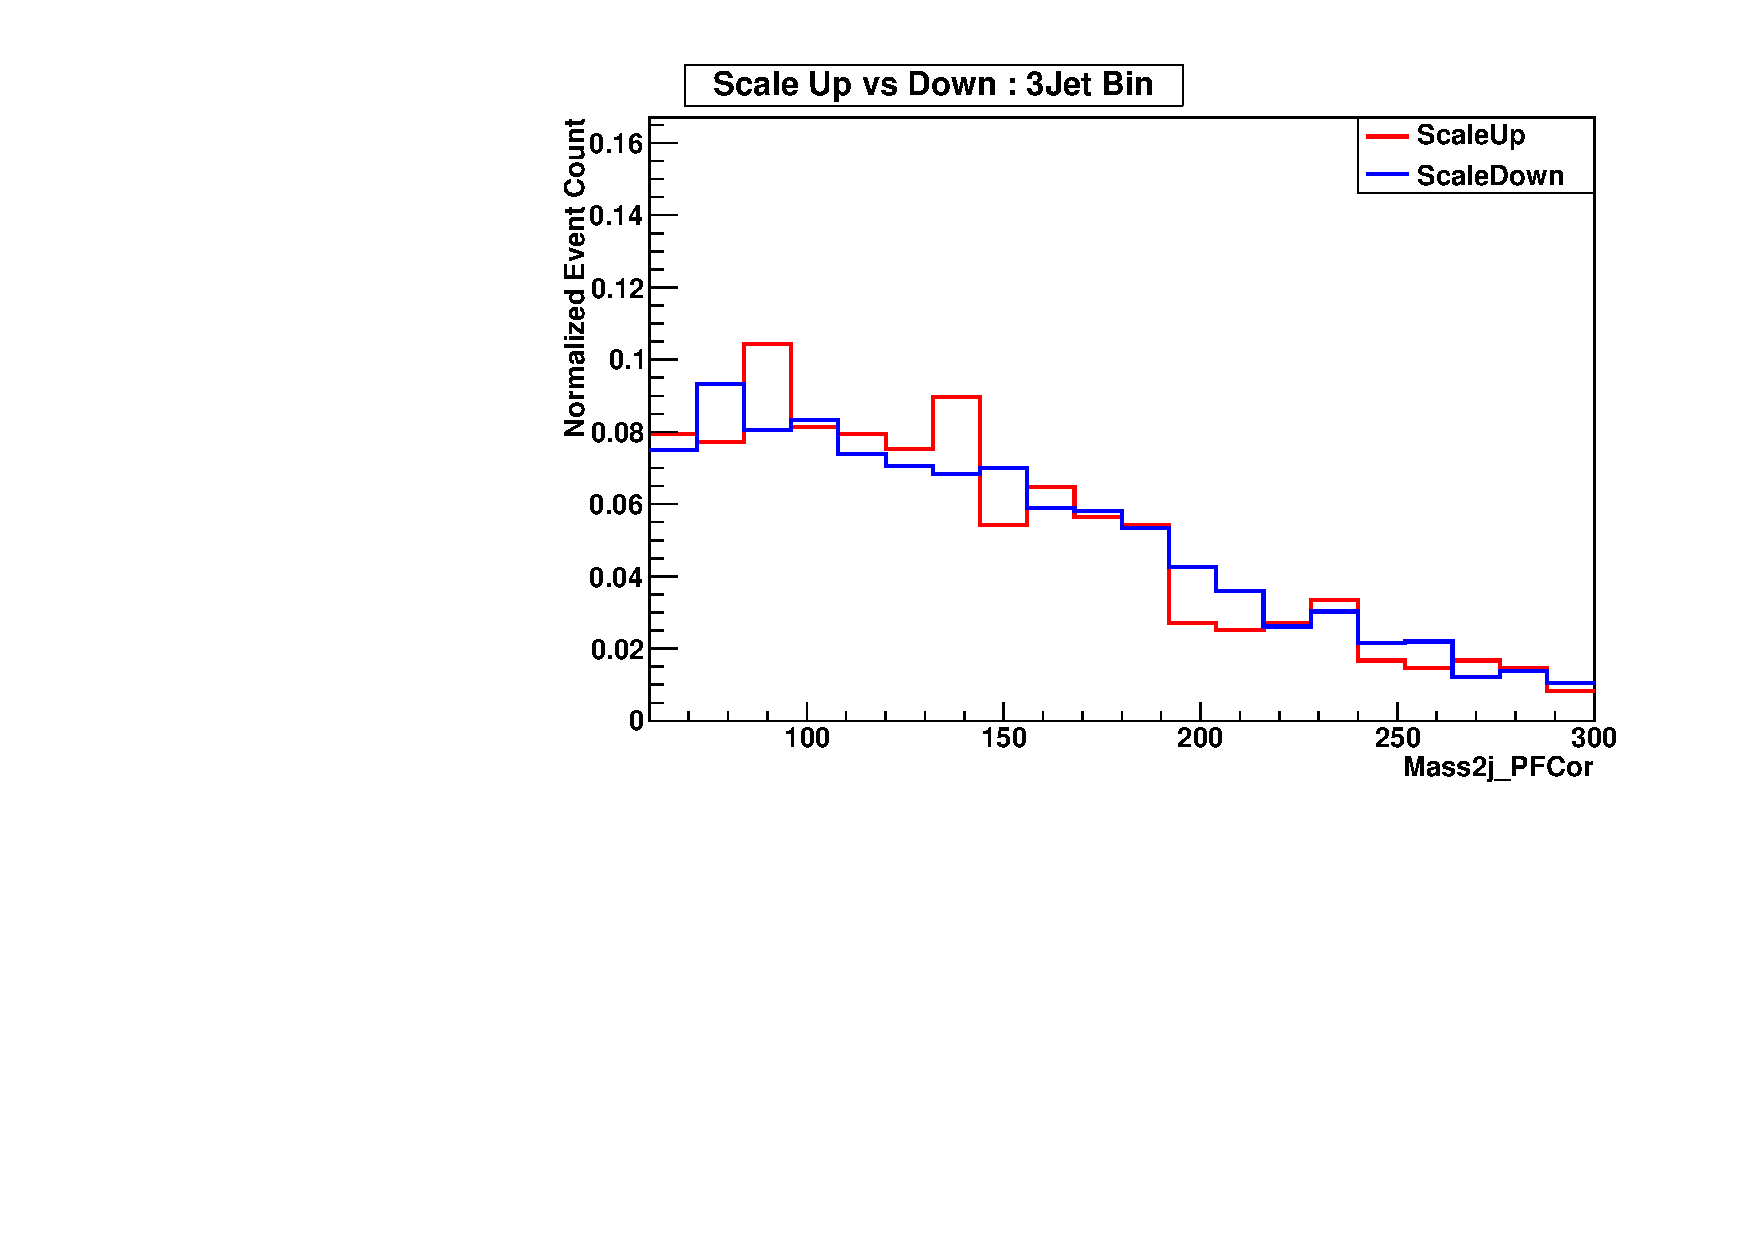
\includegraphics[width=0.48\textwidth]{figs/validation/ShapeComp_Scale3j.pdf}
\put(-0.80,0.0){(b)} \\
\unitlength=0.33\linewidth
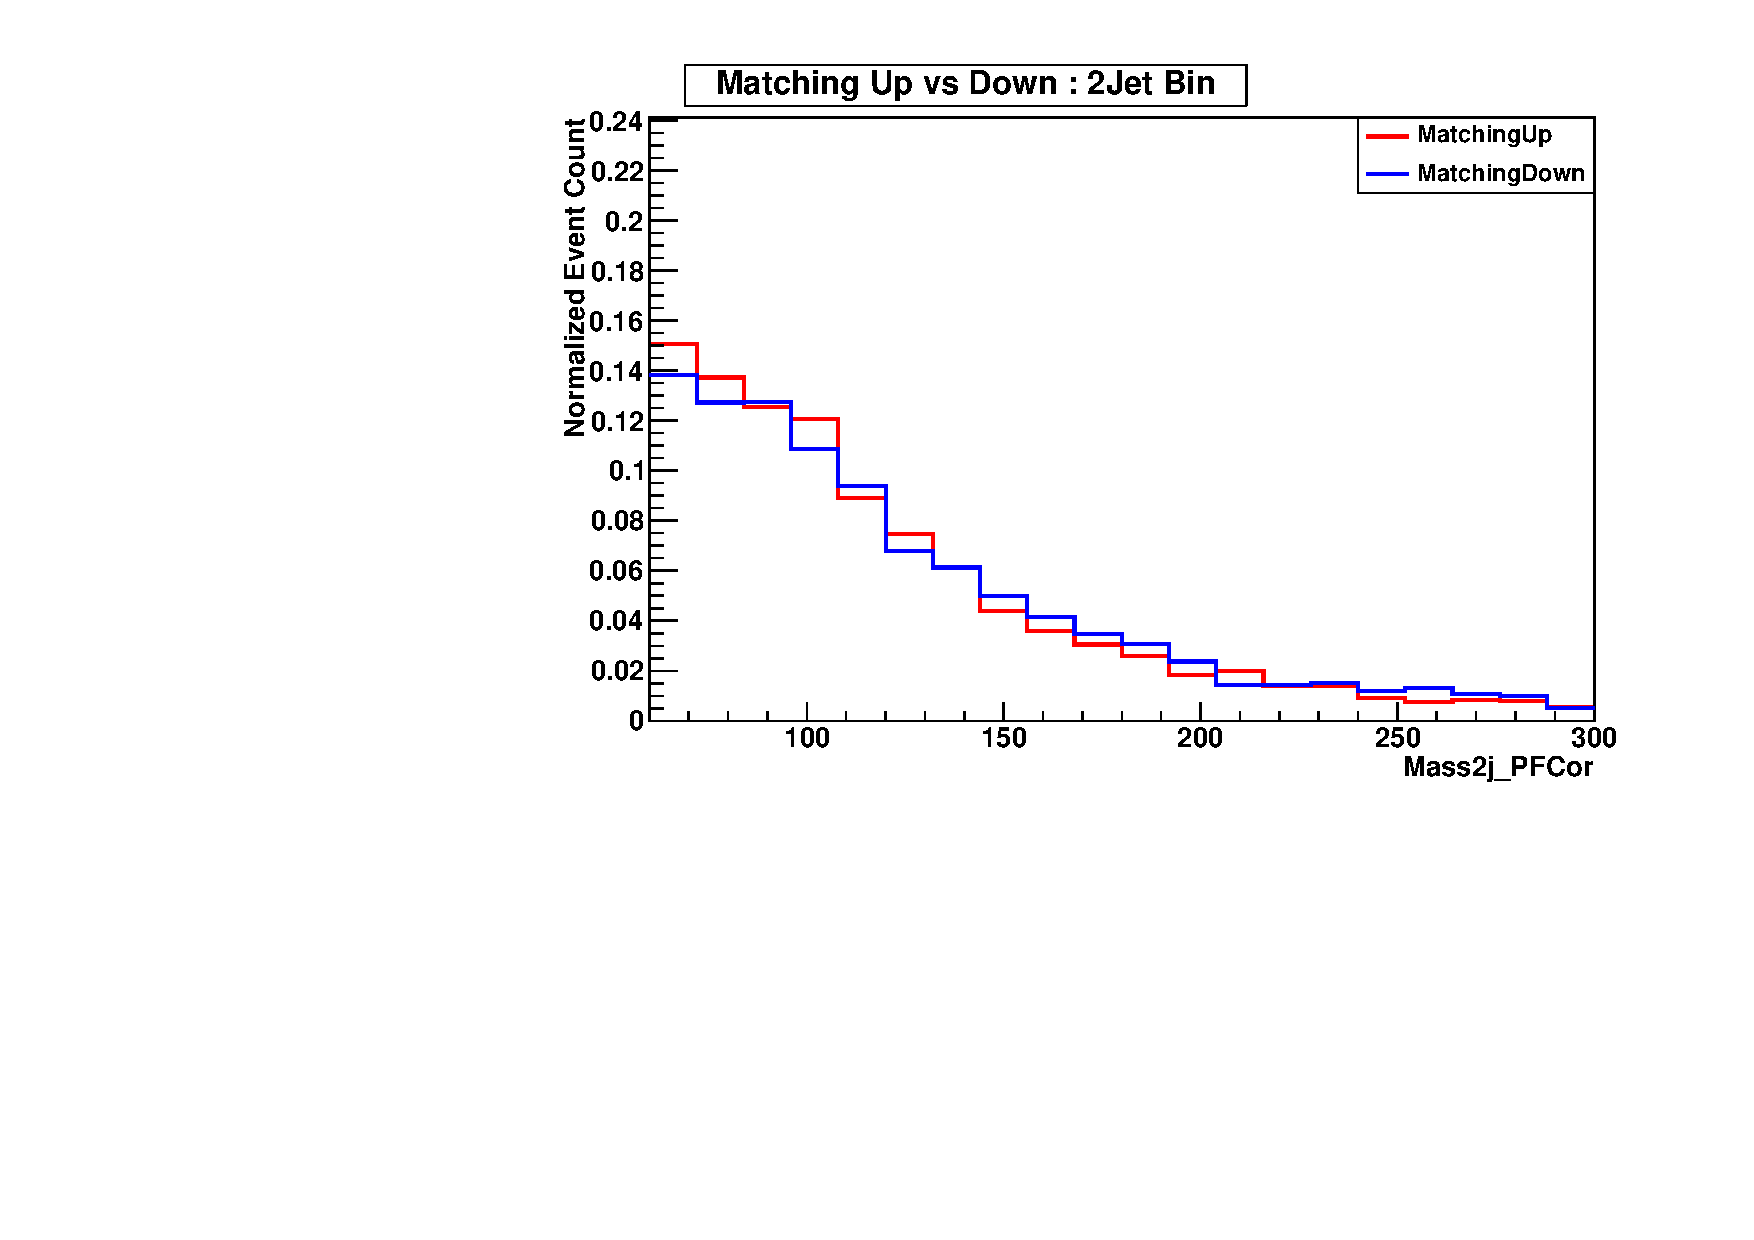
\includegraphics[width=0.48\textwidth]{figs/validation/ShapeComp_Matching2j.pdf}
\put(-0.80,0.0){(c)} 
\unitlength=0.33\linewidth
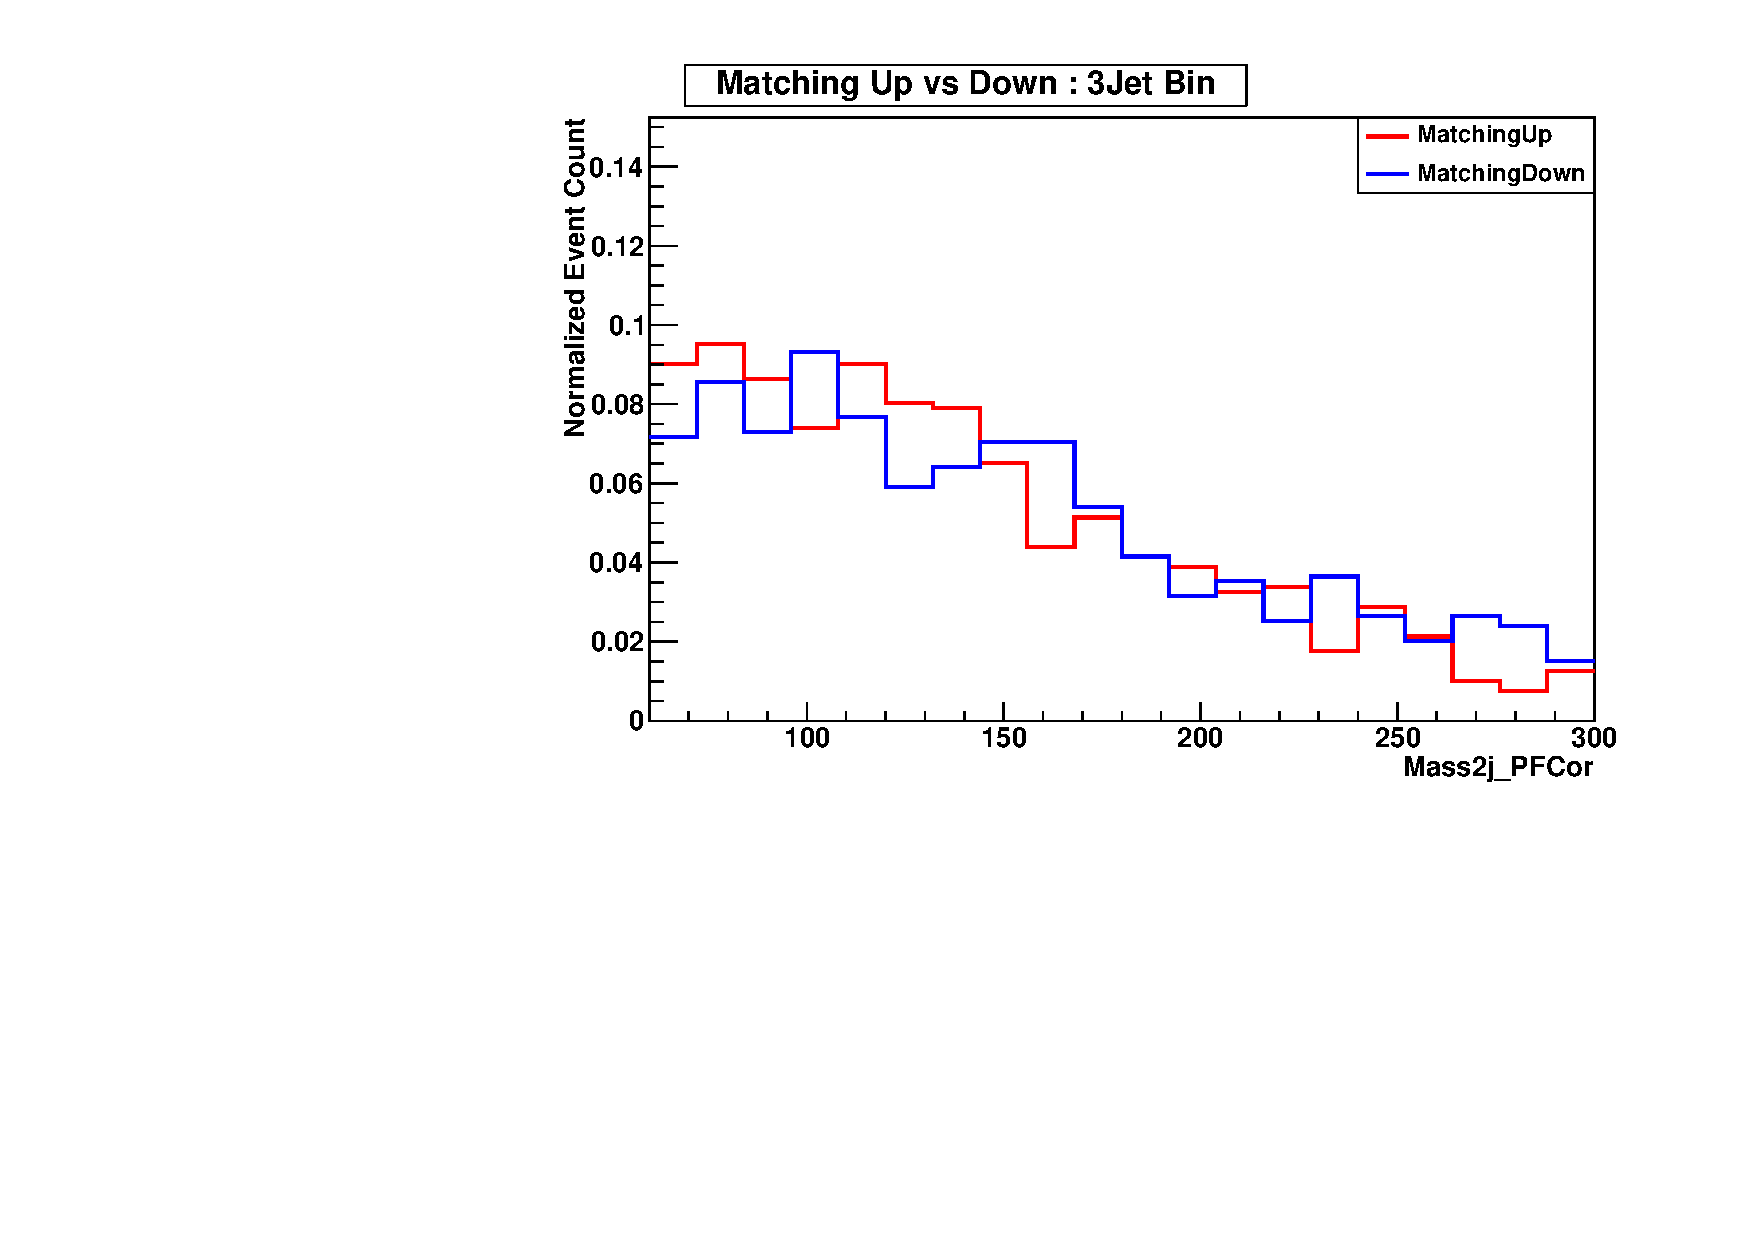
\includegraphics[width=0.48\textwidth]{figs/validation/ShapeComp_Matching3j.pdf}
\put(-0.80,0.0){(d)} 
\caption{Comparison between Up and Down shapes for: (a) scale - 2-jet bin, (b) scale - 3-jet bin, (c) matching - 2-jet bin, (d) matching - 3-jet bin.} 
\label{fig:Validation_ShapeComparisonUpVsDown}
}
\end{figure}
%%%%%%%
\begin{figure}[h!] {\centering
\unitlength=0.33\linewidth
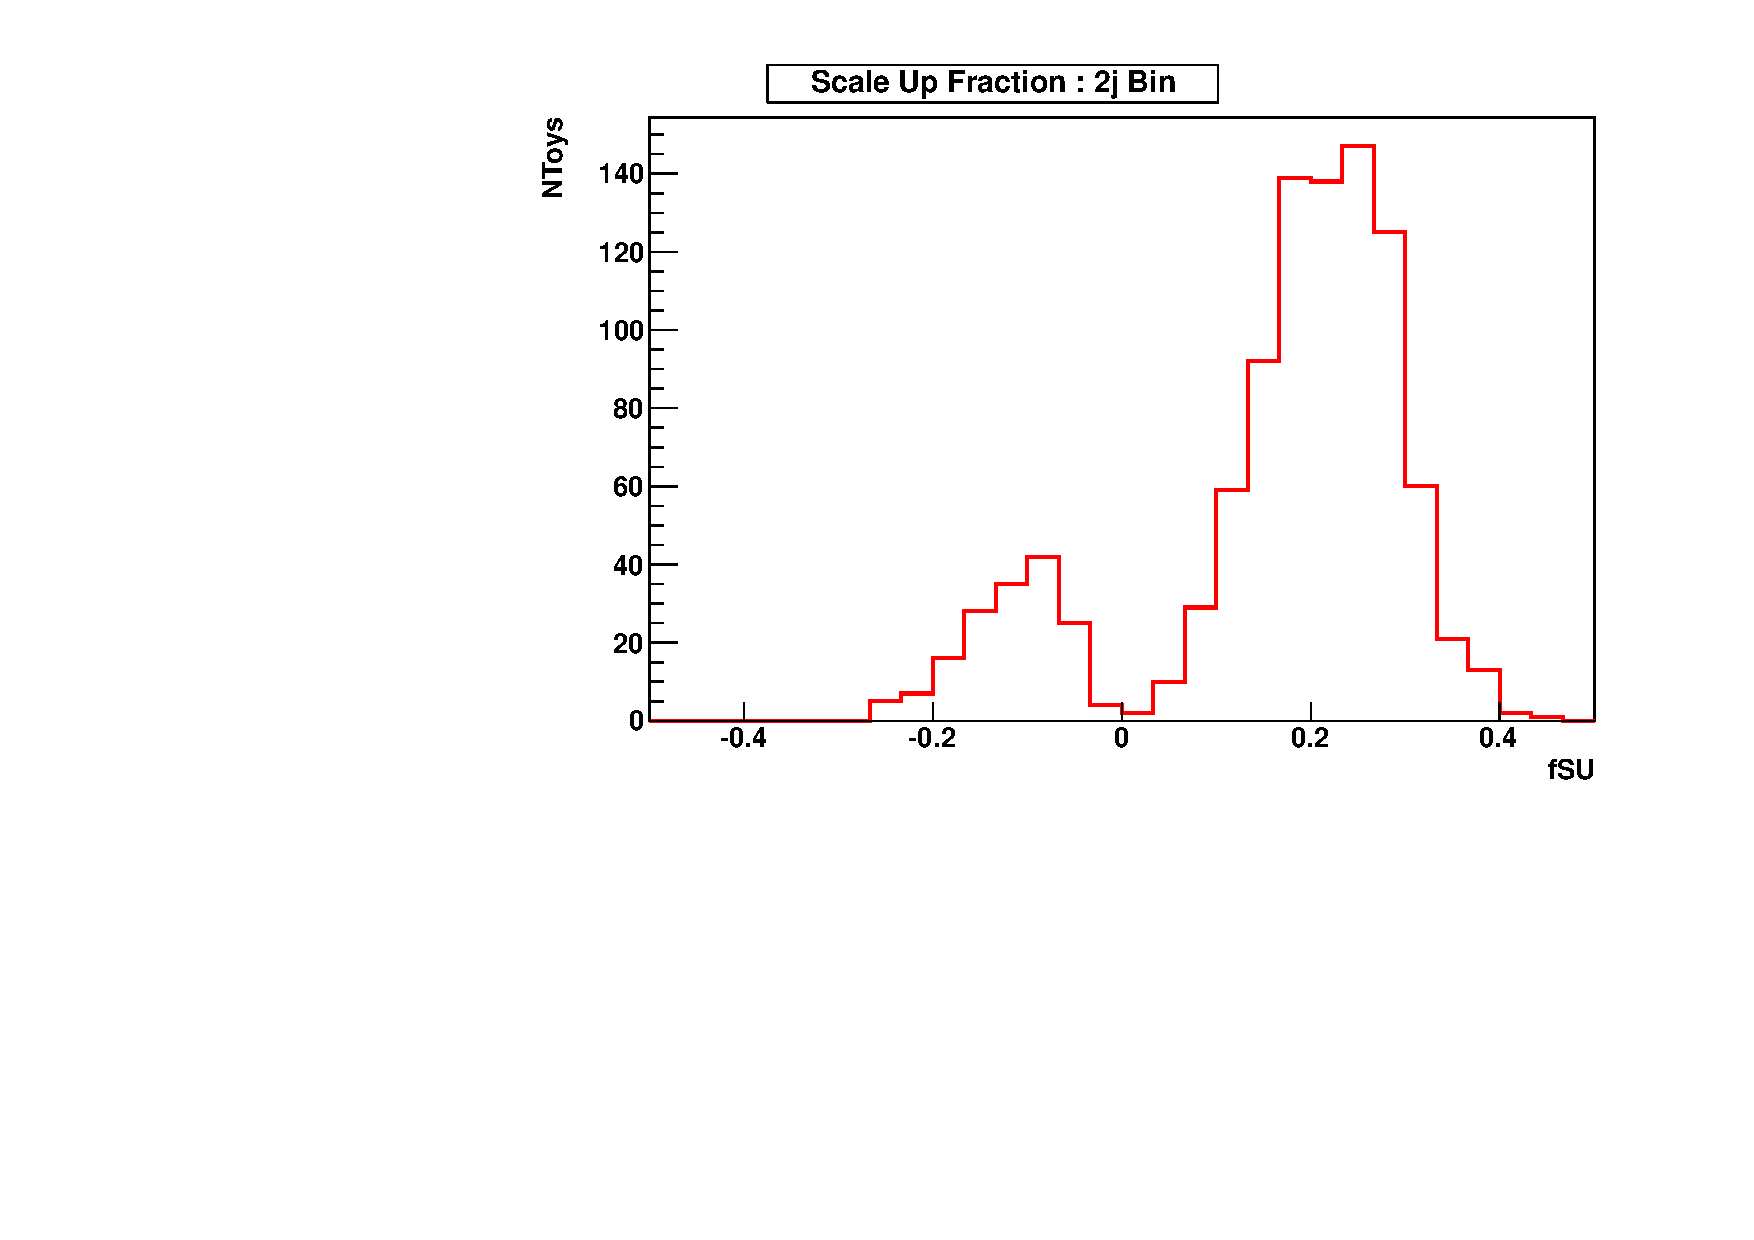
\includegraphics[width=0.48\textwidth]{figs/validation/ToyFits_fSU_2j.pdf}
\put(-0.80,0.0){(a)} 
\unitlength=0.33\linewidth
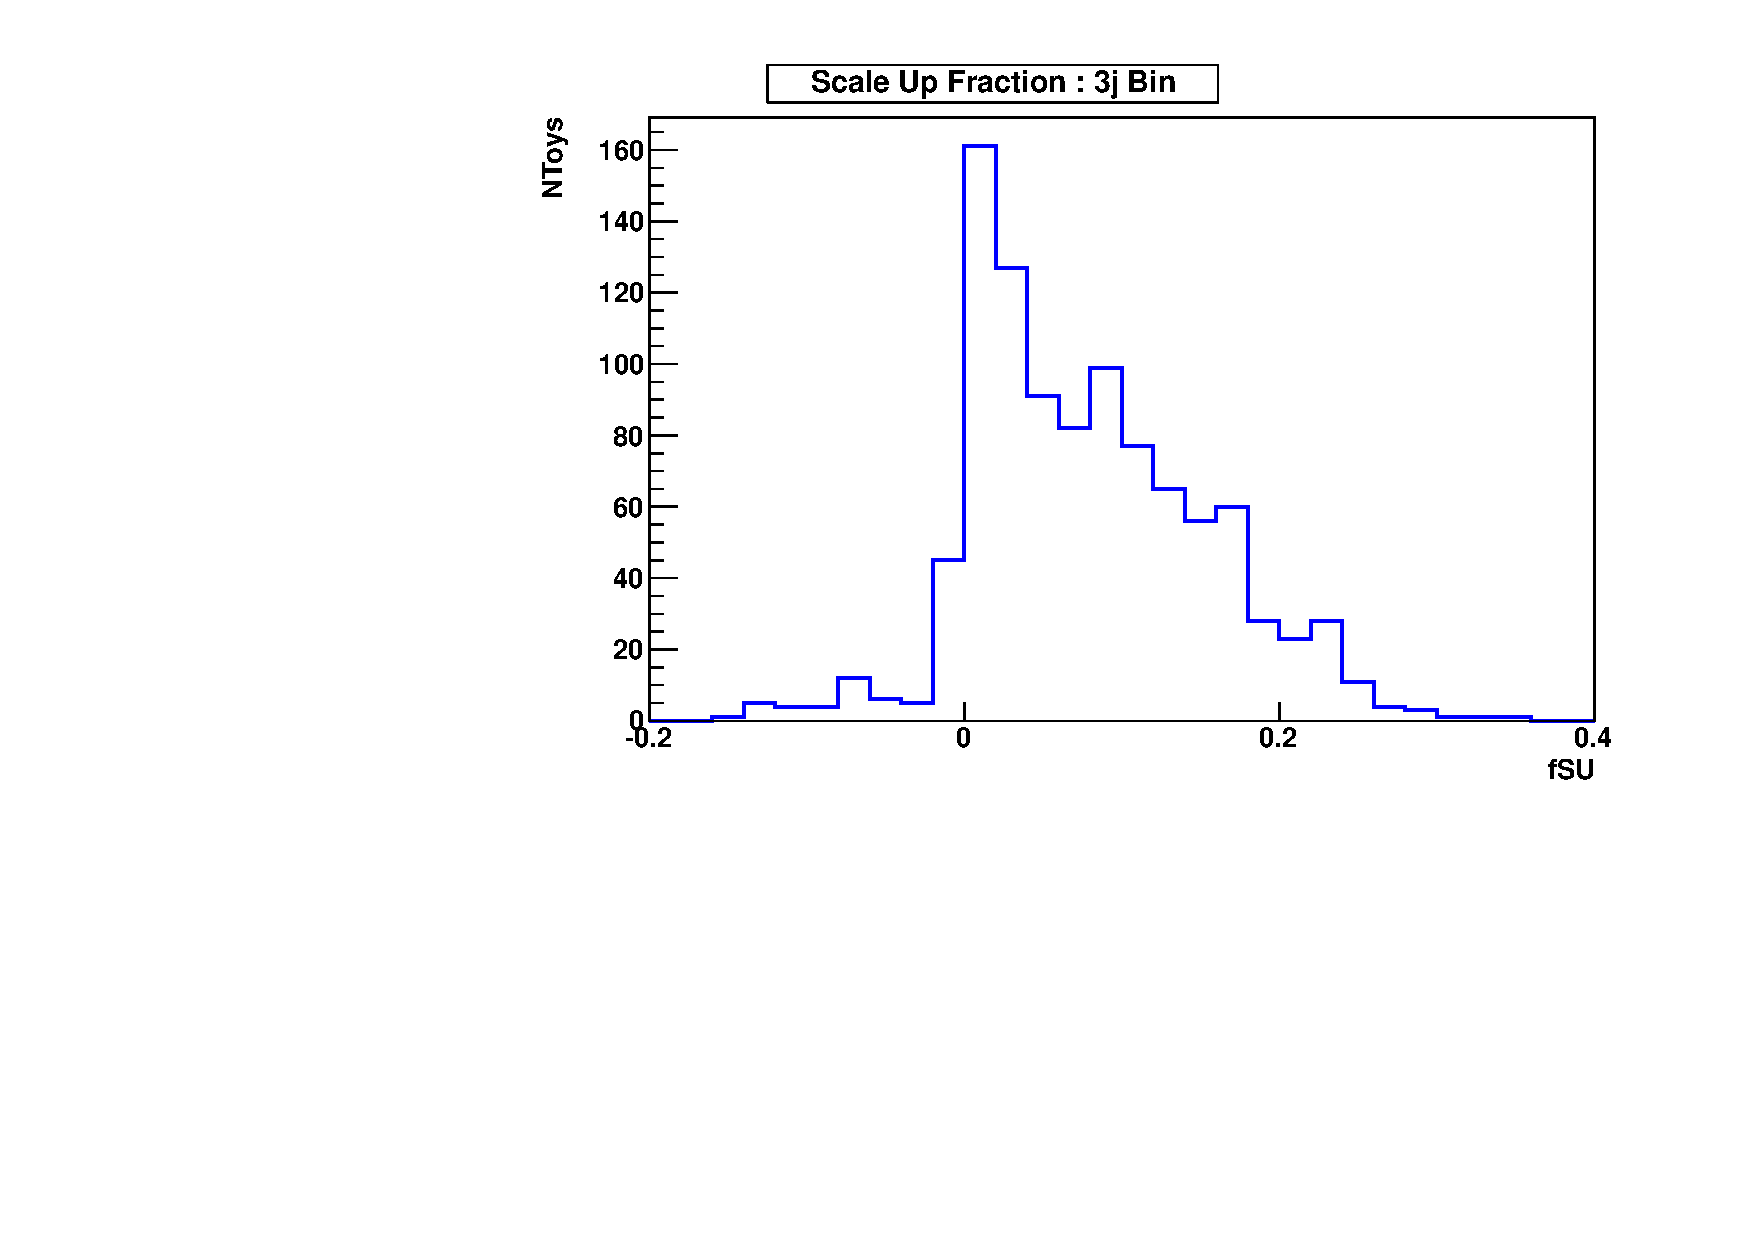
\includegraphics[width=0.48\textwidth]{figs/validation/ToyFits_fSU_3j.pdf}
\put(-0.80,0.0){(b)} \\
\unitlength=0.33\linewidth
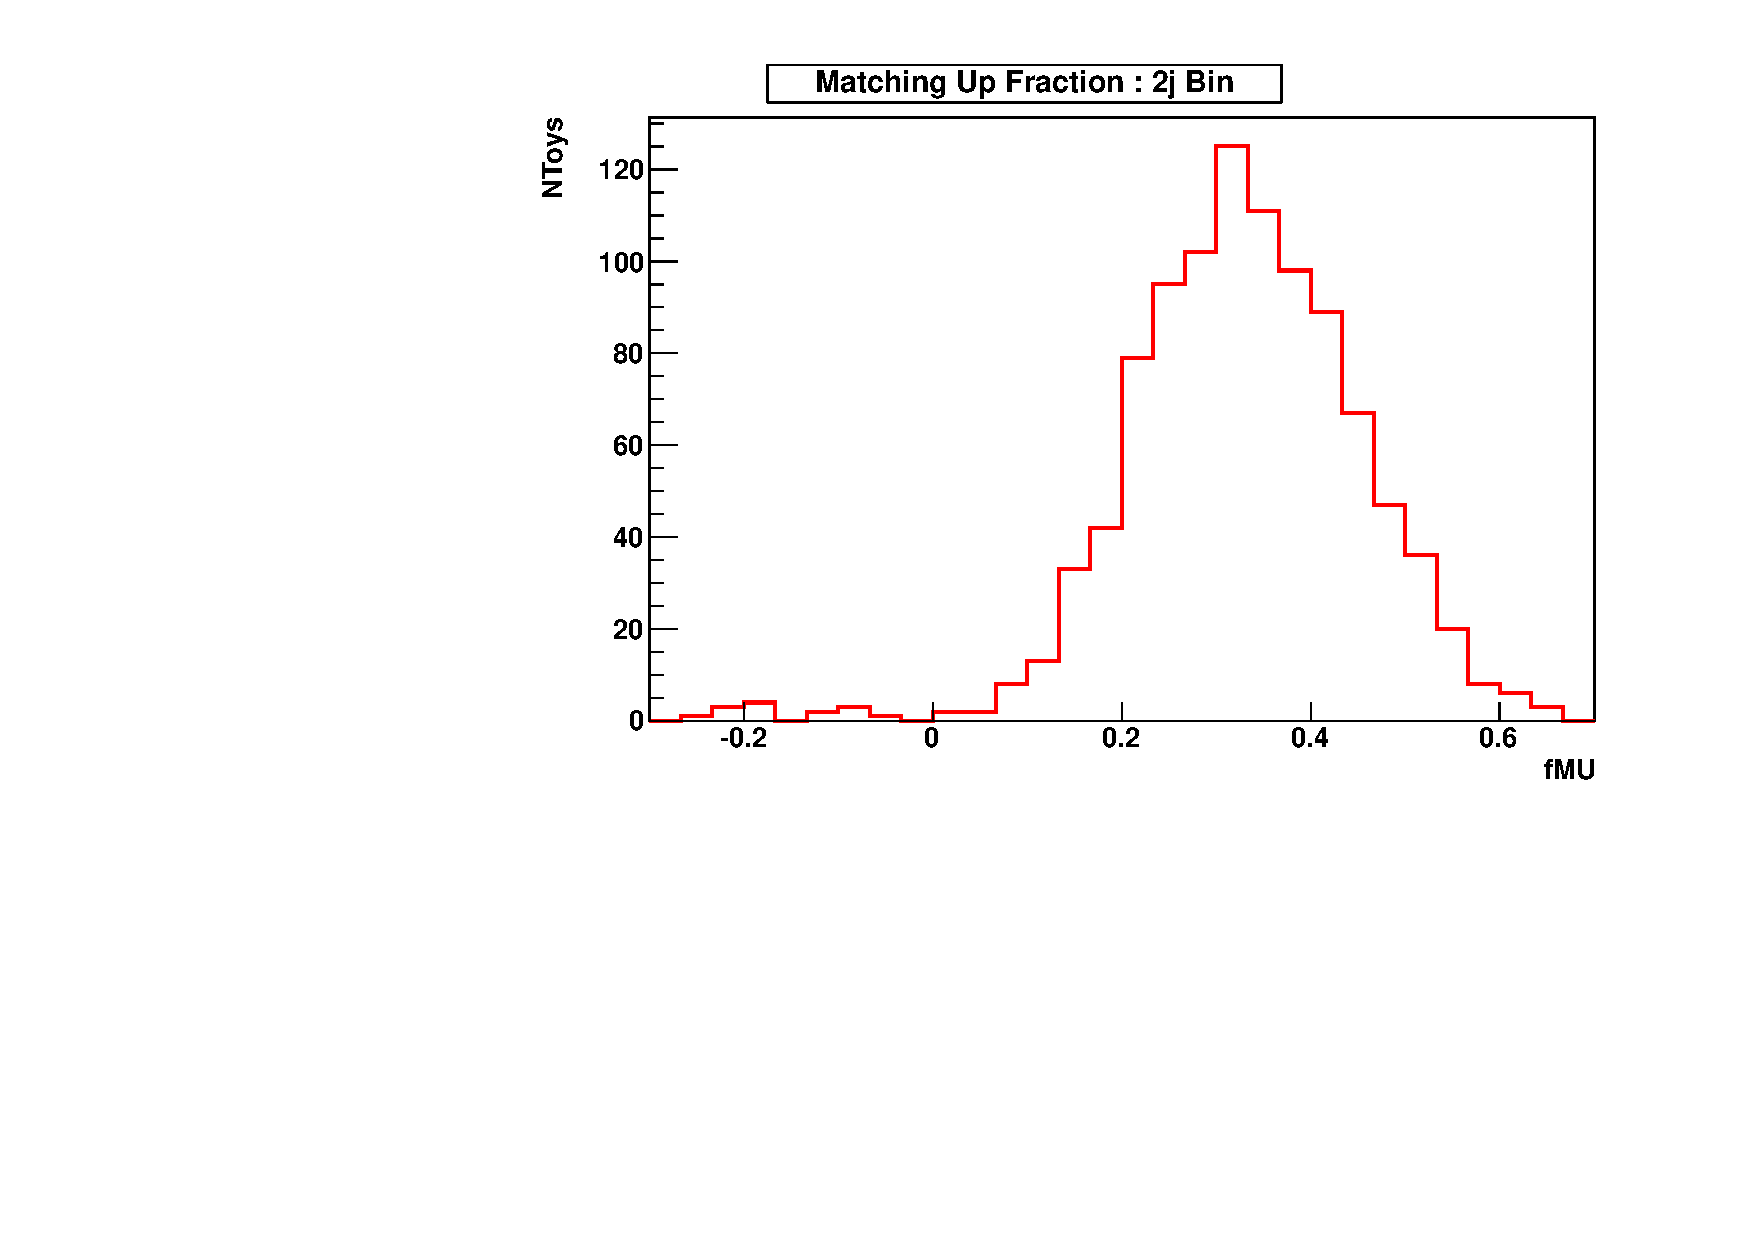
\includegraphics[width=0.48\textwidth]{figs/validation/ToyFits_fMU_2j.pdf}
\put(-0.80,0.0){(c)} 
\unitlength=0.33\linewidth
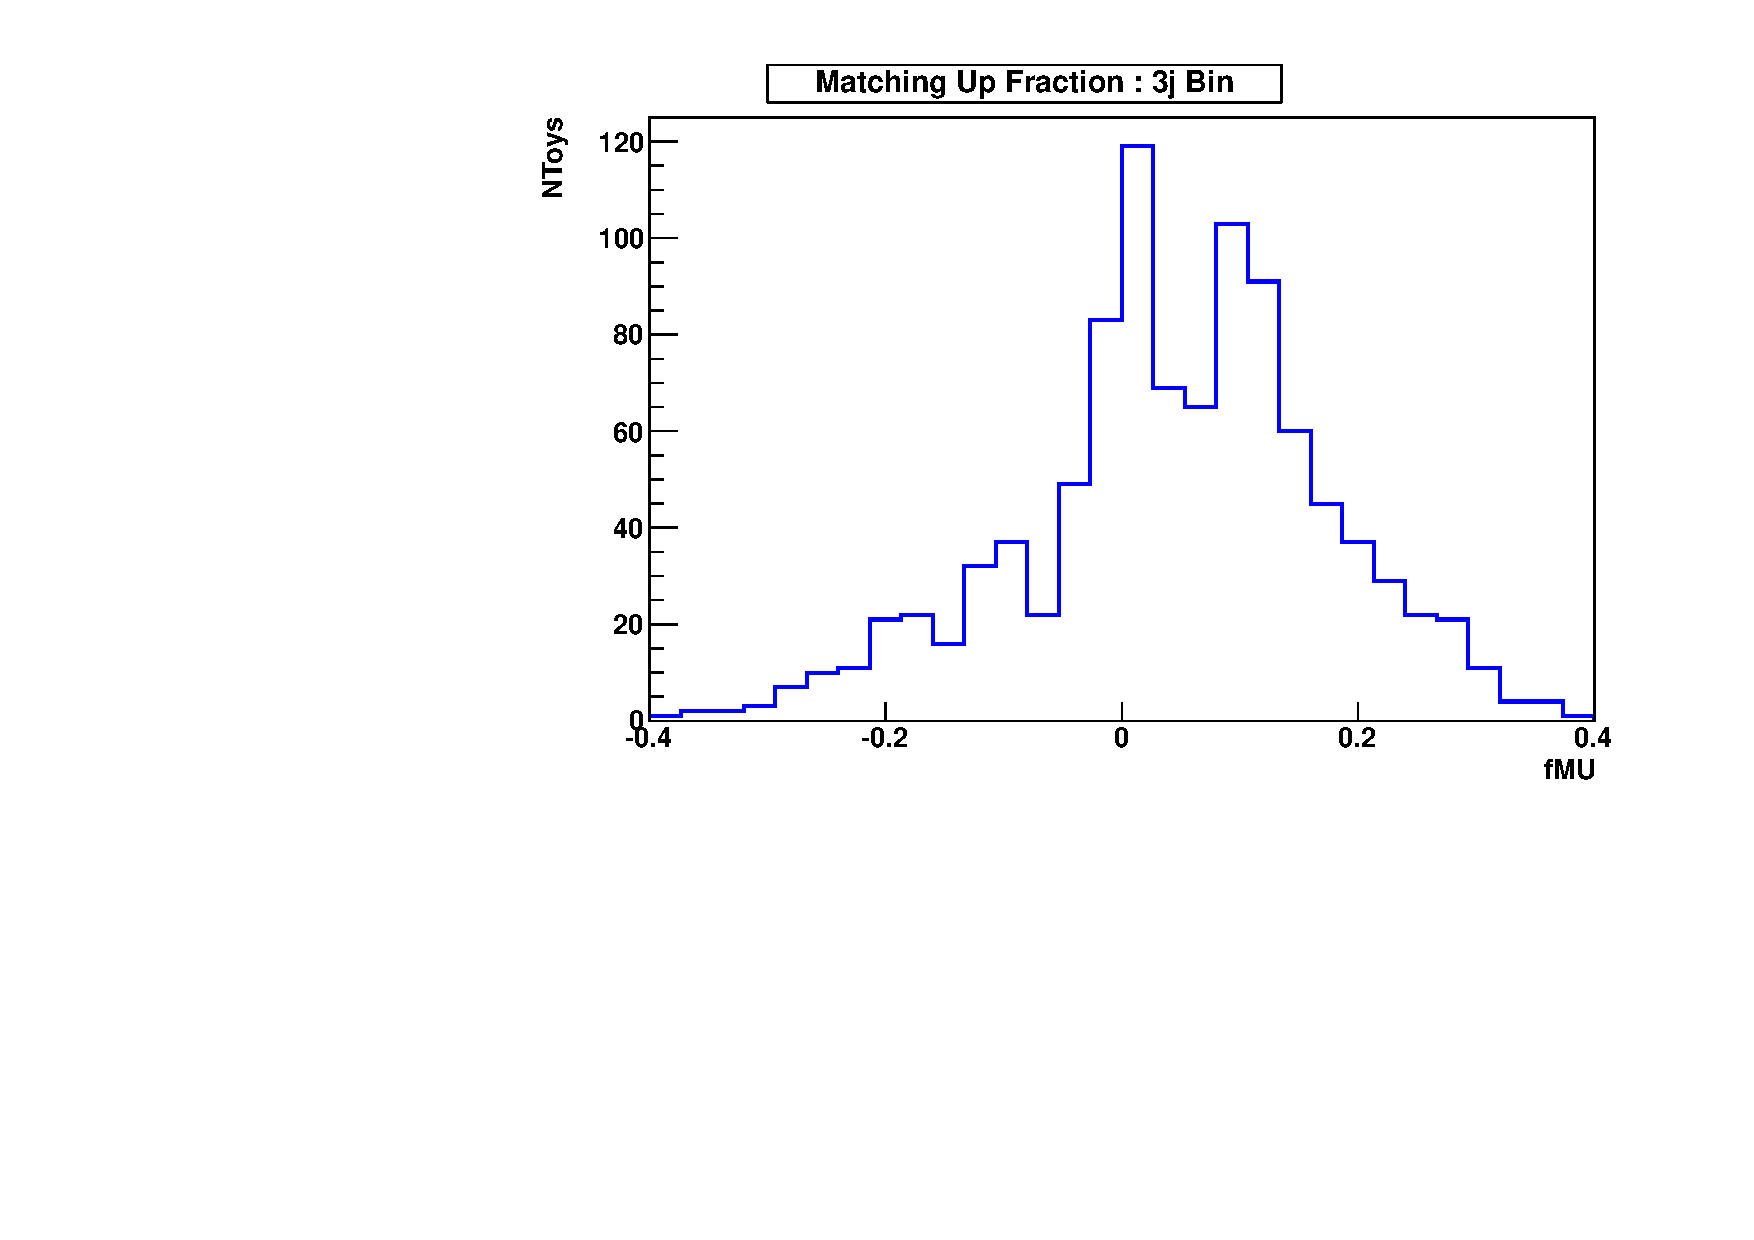
\includegraphics[width=0.48\textwidth]{figs/validation/ToyFits_fMU_3j.pdf}
\put(-0.80,0.0){(d)} 
\caption{Optimization Procedure Validation using 1000 Toy MC datasets. Most likely values for: (a) scaleUp fraction - 2-jet bin, (b) scaleUp fraction - 3-jet bin, (c) matchingUp fraction - 2-jet bin, (d) matchingUp fraction - 3-jet bin. By convention $fSU<0$ corresponds to scaleDown and $fMU<0$ corresponds to matchingDown events.} 
\label{fig:Validation_fSUfMU}}
\end{figure}
%%%%%%%
%%%%%%%%%%%%%%%%%%%%%%%%%%%%